\RequirePackage[OT1]{fontenc}
\documentclass[letterpaper,journal]{IEEEtran}
\usepackage{amsmath,amssymb}
\usepackage{cite}
\usepackage{graphicx}
\usepackage{booktabs,array}
\usepackage{algorithmic}
\usepackage{xcolor}
\usepackage{tikz}
\usetikzlibrary{arrows.meta,positioning,fit,calc}
\usepackage[hidelinks]{hyperref}
\hypersetup{pdftitle={Next: Enabling Continuous UTXO Payments with Direct Guarantees},pdfauthor={Lu Hengrun}}
\graphicspath{{figures/}{./}}
\newtheorem{theorem}{Theorem}
\newtheorem{lemma}{Lemma}
\newtheorem{definition}{Definition}
\newcommand{\Next}{\textsc{Next}}
\newcommand{\Hash}{\mathsf{H}}
\newcommand{\CAL}{\mathsf{CAL}}
\newcommand{\FUEL}{\mathsf{FUEL}}
\title{Next: Enabling Continuous UTXO Payments with Direct Guarantees}
\author{Lu Hengrun\thanks{Lu Hengrun is with University.}}
\begin{document}
\maketitle
\begin{abstract}
When UTXO recipients wait for public execution before spending, every
payment hop adds a confirmation delay. Next lets a recipient continue after
one certification round. Our insight is that the certificate traveling with
an output names who answers for a missing source: its direct issuer.
Members of the consuming organization lock inputs and reserve capacity for
all certified outputs; a recipient that verifies their quorum certificate
(TXCer) may request a successor, subject to successor admission and
capacity. If the successor executes first, public execution consumes the
certified output and records a funded obligation against that issuer.
Source execution fulfills the obligation; otherwise an included, valid post-deadline
public decision compensates the gap from the issuer's reserve, a later
source repays it, and a source that never executes leaves the loss with the
issuer. Authorized historical repair records that debit in the consuming
input under the original block identity, without re-executing payments or making economic closure wait for
historical repair. For four-member organizations and a four-validator
committee, each with at most one static Byzantine member, we prove unique
consumption, coverage of every certificate's outstanding liability, CAL
conservation, and order-independent terminal CAL holdings for finite,
acyclic, source-closed, conflict-free payment sets whose payments each
succeed exactly once. On one host with synchronous member commits and NoSync wallets, a
100-hop chain reaches its last certified receipt in a median 4.707\,s,
versus 64.479\,s with per-hop waiting.
\end{abstract}

\begin{IEEEkeywords}
Blockchain, certified payments, collateral, Byzantine fault tolerance,
chameleon hash.
\end{IEEEkeywords}

\section{Introduction}
\label{sec:introduction}

In a UTXO ledger, each payment spends outputs of earlier transactions, so if recipients wait for public execution, every hop of a payment chain adds a confirmation delay. Suppose Alice pays Bob 100 CAL and Bob forwards it to Carol before Alice's payment executes. If Bob's payment executes first, the ledger consumes an output that does not yet exist, and the missing 100 CAL needs an identified, funded source, whether Alice's transaction arrives later or never.

Waiting for public execution at every hop is the direct alternative, and our evaluation uses it as a control. Certificate-based systems separate recipient usability from public processing: FastPay and Zef support low-latency certified payments, and Sui Lutris combines broadcast and consensus paths for different kinds of state access~\cite{fastpay,zef,lutris}. Payment channels obtain rapid transfers from channel liquidity~\cite{blitz,donner}. Next asks how a native ledger can fund a certified payment whose source has not executed, with registered organizations rather than channels standing behind it.

Three difficulties are coupled. Certificates circulate before public registration, so accounting from public gaps misses existing commitments. A late source must not pay both the guarantor that advanced the value and the recipient who already spent it. A client may hold a source and never submit it.

Our insight is that the party answerable for a missing source is already named by the certificate that travels with the output. Next charges the gap to that direct issuer instead of tracing ancestors, bounds every signed certificate's liability by reserve-backed signing capacity, and closes an unresolved obligation by a public decision without changing stored history.

Economic closure leaves a separate record question. After compensation, the
consuming input in the original block still cites the source output that
the reserve replaced. Local exception review and historical re-export work
from stored blocks: an archival replica revisits the input, reports the
reserve advance with its authorizing decision and repayment status, and
exports the block. Authorized historical repair lets the exported body
itself name the reserve debit at the input's original coordinates. A
decision index gives the same economic answer from the original body; the
additional interface is a revised body that verifies against the original
commit, with authorization drawn from the replica's executed prefix. Ledger
auditing revisits records through saved execution evidence~\cite{ia-ccf},
and Reparo returns repaired data through an old transaction
hash~\cite{reparo}; Next authorizes a replacement body that keeps the
complete identity referenced by existing commits and successor
headers~\cite{comet-blockid}, without executing the payment again.

The design has three complementary contributions.

\noindent\textbf{C1: A layered architecture for one-round continuation.} A certificate
fixes a payment's outputs and names its issuer; public execution decides
which payment the ledger accepts. Before signing, each member of the
consuming organization locks the inputs and reserves capacity for all CAL
outputs, change included, in one atomic step, and one parallel round yields
a TXCer. The recipient verifies and records the output and can request a
successor at once, carrying only the certificates of its direct inputs,
while replication and public submission continue in the background.
Table~\ref{tab:model-contract} states the guarantee of each stage.

\noindent\textbf{C2: Direct responsibility with source decoupling.} When a successor
consumes a certified output whose source has not executed, public execution
records the consumption and an obligation against the direct issuer in one
atomic step. The successor's block exposes the source certificate, so the
original signers can resubmit the source from their stored approvals. After
the deadline, an included valid decision compensates the gap from the issuer's
reserve, and a late source repays it. We prove that signing capacity covers
the outstanding CAL liability of every certificate, published or not,
extending overlapping per-member budgets~\cite{stingray} to compensation
and repayment.

\noindent\textbf{C3: Authorized historical repair.} After compensation, the original
block still cites the missing source output, although the reserve funded
it. Restricted chameleon-hash commands write the reserve-debit reference
into that input. A committed compensation decision and an exact revision
task authorize each replacement; owner authorizations, output and successor
references, and the complete BlockID remain unchanged, and the commands
write representation state alone. The original commands remain the replay
history. An archival replica can then review the exception and re-export
the revised body under its existing identity, while economic closure
proceeds without waiting for the repair.

On one M4 Max host with synchronous member commits and NoSync wallet
stores, a 100-hop chain reaches its last certified receipt in a median
4.707\,s, versus 64.479\,s when waiting for public execution between
hops. On the same current build, three fourteen-service P runs complete
21,048 payments; compensation and repayment finish before paused
adaptation services resume. Separate experiments characterize behavior
under injected network delays and single faults, and the local reading,
storage, and maintenance costs of optional historical representation.

\section{Background and Related Work}
\label{sec:related}

Next combines certified payments that a recipient can reuse before public
execution, reserve-backed responsibility for a source that has not executed,
and authorized editing of stored history. We compare prior work along two
questions: who answers for a missing source, and which payment and block
identities survive once that answer is recorded.

\noindent\textbf{Certificate-based payments and execution.}
FastPay uses Byzantine consistent broadcast for low-latency payments and, in
its primary-ledger deployment, backs redemption with prepaid
funds~\cite{fastpay}. Its redeemability argument lets a valid certificate be
confirmed before all incoming transfers are locally confirmed, provided the
sender's missing earlier outgoing certificates are supplied; redemption then
reaches the primary funding pool. Zef combines disposable accounts with
private, transferable coins, and ordinary spending uses current coin
certificates and consumption evidence in place of the full ancestor
history~\cite{zef}. Sui Lutris pairs broadcast execution for owned objects
with consensus for shared-object interactions~\cite{lutris}.

Stingray supports concurrent transactions through Byzantine bounded counters
and FastUnlock~\cite{stingray}. Its overlapping per-replica budgets
(Sec.~4.2) and its treatment of budget exhaustion when no quorum certificate
forms (Sec.~5.3) are the counting precedent for Next's signing-capacity
accounting, and we do not present them as new. Its commutative workloads
differ from a payment chain in which each transaction consumes its
predecessor's output. For that chain, Next publicly executes a certified
consumption before the source executes and registers a funded obligation
against the direct issuer. It adds responsibility for certificates that were
never published, dynamic conservation of the Paid, Recovered, and Remaining
quantities of each certificate, and closure of the source obligation by a
public decision. The successor's execution also publishes the source's
certificate, so the issuing organization's own members can resubmit the
source from the approvals they stored.

\noindent\textbf{Channels and collateralized guarantees.}
Blitz replaces two-phase commitment in channel payments with
pay-or-revoke~\cite{blitz}, Donner develops virtual channels that address the
Domino attack~\cite{donner}, and CryptoMaze provides atomic multipath channel
payments with unlinkable partial payments~\cite{cryptomaze}. All three operate
through channel arrangements. Next runs on a native ledger with registered
consumption routes and organization reserves, so counterparties need neither a
bilateral channel nor a prefunded route between them.

Snappy protects merchants who accept fast on-chain payments through
collateralized approvals, and reusable payment guarantees combine privacy with
customer collateral that can be reused across defined time
windows~\cite{snappy,reusable}. The service trigger differs: FastPay backs primary-ledger redemption
with prepaid funds, and Snappy gives an accepting merchant a collateral claim
under its approval rules. In Next, signing reserves issuer backing, but the
public obligation arises when an executed successor consumes a missing
certified output. Compensation closes that source obligation without a second
principal credit to the child recipient. A terminal holder whose source never
executes and who has no executing successor has no certificate-only redemption
path (Section~\ref{sec:model-contract}). HyperService adjudicates cross-chain
execution violations through a public Network Status Blockchain and an
Insurance Smart Contract that financially reverses the effects of committed
transactions~\cite{web3}. Next draws the responsibility boundary within one
native UTXO ledger: compensation settles a direct issuer obligation and leaves
the principal effects of executed successors in place.

\noindent\textbf{Controlled editing and historical consistency.}
Chameleon hashes permit authorized alternative messages under the same digest
and underpin editable-blockchain designs~\cite{redactable}. SDR studies
decentralized attribute-based edit authority and dynamic
delegation~\cite{sdr}, Escaping moves committee selection and voting outside
the consensus layer to shorten redaction waiting~\cite{escaping}, and
Reconstructing Chameleon Hash develops stronger definitions of
indistinguishability and collision resistance~\cite{reconstructCH}. Next uses
an established adaptation primitive, with the trapdoor held as threshold
shares of an RSA exponent following Shoup's practical threshold-signature
approach~\cite{shoup}. The authority to apply a compatible replacement comes
from a committed compensation decision and public payment-state checks, not
from the primitive.

Reparo provides a publicly verifiable repair layer and can re-execute affected
transactions while repairing state~\cite{reparo}. Its Ethereum implementation also maps an old transaction hash to
repaired transaction data, supporting access through an existing record
identifier. IA-CCF audits immutable ledger records against saved execution
receipts~\cite{ia-ccf}. These systems motivate review through established
record references; Next specializes the revision authority to a committed
compensation decision. Next fixes payment
authorizations and outputs in advance: a public decision accounts for the
compensation once, and representation commands replace only the permitted
funding representation, without re-executing successors. The original
commands, including the decisions, remain the economic replay history.
RedactChain coordinates concurrent edits to the same block and their
preprocessing~\cite{redactchain}, and CDEdit uses reusable privilege tokens to
cut repeated token and key generation and verification across multiple
edits~\cite{cdedit}. In Next, a batch shares the final block representation
across the decided slots of one block, and each slot's reserve debit was
already committed by its own decision, so the edit has no economic effect. The
complete block identity combines the stable header hash with the original
part-set header, and publicly committed logical revisions authorize exact
replacement bodies. Physical installation can therefore advance directly to a
later authorized revision without changing successor references or replay of
the public command history.

\section{System Model and Overview}
\label{sec:model}
\begin{figure*}[t]
\centering
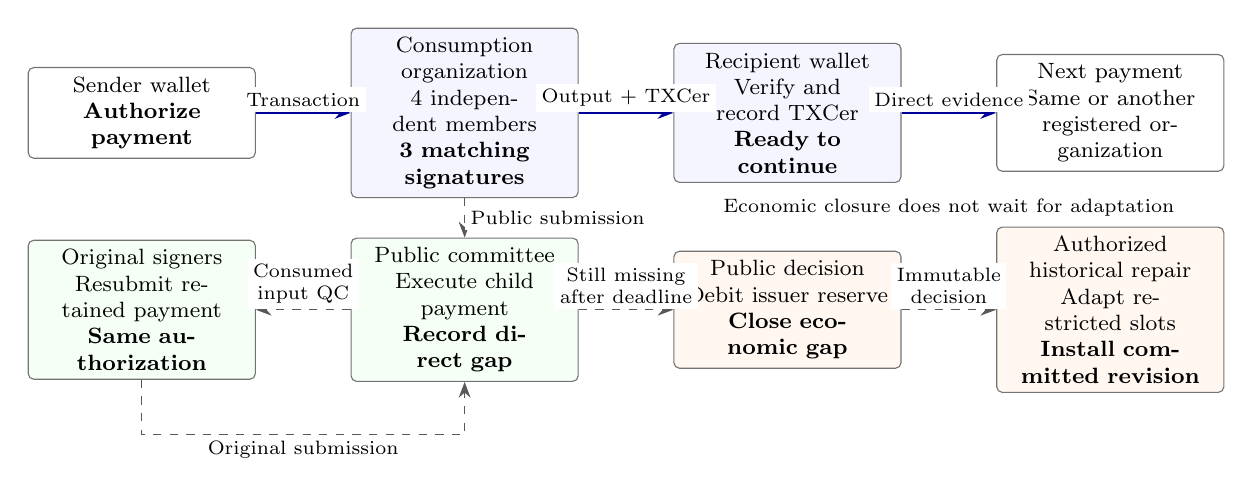
\begin{tikzpicture}[x=1cm,y=1cm,font=\footnotesize,
box/.style={draw=black!55,rounded corners=2pt,align=center,minimum height=1.05cm,text width=2.65cm,fill=white},
flow/.style={-{Stealth[length=2mm]},thick,draw=blue!60!black},
bgflow/.style={-{Stealth[length=2mm]},draw=black!65,dashed},
lab/.style={font=\scriptsize,align=center,fill=white,inner sep=2pt}]
\node[box] (sender) at (0,0) {Sender wallet\\\textbf{Authorize payment}};
\node[box,fill=blue!4] (org) at (4.1,0) {Consumption organization\\4 independent members\\\textbf{3 matching signatures}};
\node[box,fill=blue!4] (wallet) at (8.2,0) {Recipient wallet\\Verify and record TXCer\\\textbf{Ready to continue}};
\node[box] (next) at (12.3,0) {Next payment\\Same or another\\registered organization};
\draw[flow] (sender) -- node[lab,above]{Transaction} (org);
\draw[flow] (org) -- node[lab,above]{Output + TXCer} (wallet);
\draw[flow] (wallet) -- node[lab,above]{Direct evidence} (next);
\node[box,fill=green!4] (recover) at (0,-2.5) {Original signers\\Resubmit retained payment\\\textbf{Same authorization}};
\node[box,fill=green!4] (comm) at (4.1,-2.5) {Public committee\\Execute child payment\\\textbf{Record direct gap}};
\node[box,fill=orange!6] (decision) at (8.2,-2.5) {Public decision\\Debit issuer reserve\\\textbf{Close economic gap}};
\node[box,fill=orange!6] (repair) at (12.3,-2.5) {Authorized historical repair\\Adapt restricted slots\\\textbf{Install committed revision}};
\draw[bgflow] (org) -- node[lab,right]{Public submission} (comm);
\draw[bgflow] (comm) -- node[lab,above]{Consumed\\input QC} (recover);
\draw[bgflow] (recover.south) -- ++(0,-.7) -| node[lab,pos=.25,below]{Original submission} (comm.south);
\draw[bgflow] (comm) -- node[lab,above]{Still missing\\after deadline} (decision);
\draw[bgflow] (decision) -- node[lab,above]{Immutable\\decision} (repair);
\node[lab] at (10.25,-1.2) {Economic closure does not wait for adaptation};
\end{tikzpicture}
\caption{One-round continuation and evidence-driven source resolution. Solid arrows form the recipient path; dashed arrows denote background work. Public successor evidence enables the original signers to resubmit retained authorized material. If the source remains unresolved after its deadline, an included valid decision closes the gap independently of adaptation. A subsequent authorized historical repair preserves the payment and complete block identities.}
\label{fig:architecture}
\end{figure*}


Next lets a recipient spend a newly certified output before the transaction that creates it executes publicly. Four objects carry the design: authenticated payment rights, their public consumption, the responsibility for unresolved sources, and the later representation of that responsibility in stored history. Table~\ref{tab:model-notation} lists the notation.

\begin{table}[!b]
\caption{Principal notation.}
\label{tab:model-notation}
\centering
\begin{tabular}{@{}p{0.23\columnwidth}p{0.69\columnwidth}@{}}
\toprule
Symbol & Meaning \\
\midrule
$G,\mathcal C$ & Guarantor organization and public committee \\
$T,c_T$ & Payment and its certified summary fact \\
$(x,i)$ & Output identifier and spend instance \\
$g,B_g$ & Grant and cumulative authorization \\
$a_T,p_T,\mathsf{Rec}_T$ & Total CAL outputs, gross compensation, and recovered compensation \\
$\mathcal O_x,\mathcal D_x$ & Direct obligation for a missing output and its immutable compensation decision \\
$(H_b,P_b)$ & Stable block hash and original part-set header \\
$\rho_\ell,\rho_p$ & Committed logical and installed physical revisions \\
\bottomrule
\end{tabular}
\end{table}

\subsection{Participants, Assets, and Assumptions}
\label{sec:model-participants}
Next operates a native UTXO ledger. CAL carries payment value and FUEL pays processing fees. Users spend their own outputs, and organizations hold additional CAL in public reserve accounts. The fast path requires an output with a supported organization route; payment principal stays with its owner, and no bilateral channel is opened. Fees default to the user's final FUEL outputs; an authorized organization-funded mode also exists.

Each organization has four fixed members and a replaceable collector. Members validate requests independently and authorize payments, while the collector distributes requests, assembles certificates, and coordinates propagation without spending authority. A separate committee $\mathcal C$ of four equally weighted validators, with three votes required, orders public commands and maintains accounts, outputs, obligations, and compensation decisions.

\noindent\textbf{Faults and cryptography.}
The adversary corrupts statically at most one member per organization and one committee validator throughout an execution; users and collectors behave arbitrarily. Honest participants share the network configuration, genesis, rules, and organization registry, and each route names one active configuration and one consumption-lock domain. Signatures are unforgeable, canonical digests and original block commitments are binding, and messages may be delayed arbitrarily.

\noindent\textbf{State.}
Honest signing state is atomic and never forgotten or rolled back. Before a member signs, its approval records the payment, the admission vector, and the direct input certificates of the request; the quorum certificate is not part of it. Public execution is deterministic and atomically committed, and followers apply authenticated consecutive blocks, updating state and cursor together. Compensation and representation read original blocks and their metadata, so correct committee replicas retain both at every height that holds an open obligation or a decided slot awaiting representation.

\noindent\textbf{Adaptation and progress.}
Representation uses threshold adaptation with material generated and distributed by a trusted offline dealer, and a committed command must authorize any adaptation output. Progress needs responsive honest participants, available evidence, sufficient fees and resources, and fair delivery and scheduling. The experimental in-memory configuration keeps state atomic only while the process runs, and each run starts from fresh genesis.

Historical reads concern an honest replica that has verified and executed public prefix $H$, using one read transaction on its state $V_H$. Section~\ref{sec:protocol-reader} specifies the interface semantics.

\subsection{A Continuous-Payment Example}
\label{sec:model-example}
Alice pays Bob 100~CAL through organization $G_A$, creating output $x$
routed to $G_B$. The payment passes through three stages, whose guarantees
Table~\ref{tab:model-contract} lists.

\emph{Certified receipt.} Members of $G_A$ lock Alice's inputs, reserve
signing capacity for every CAL output of her payment, change included, and
sign; three matching signatures form the TXCer. Bob verifies it and records
$x$. He can then ask $G_B$ to certify a payment to Carol, which $G_B$
admits under its own input, fee, and capacity checks. At this stage Bob
holds an authenticated right to request continuation, before any public compensation obligation is created.

\emph{Public consumption.} If Bob's payment executes before Alice's, the
committee consumes $(x,0)$, records a 100-CAL obligation against $G_A$, and
creates the outputs of Bob's payment as final, all in one transition. Carol
spends her output under the ordinary final-input rules. The same block
carries the certificate of Alice's payment, so members of $G_A$ that
approved it can resubmit it when Alice's wallet does not.

\emph{Economic closure.} If Alice's payment executes while the obligation is
Open, it fulfills the obligation. Once the deadline set by public block time
has passed, a public decision can instead debit $G_A$'s reserve by 100~CAL
and mark the obligation Compensated (the implementation's \texttt{Repaired}
status). Carol receives no second credit, and Bob's payment executes only
once. If Alice's payment executes afterwards, it repays $G_A$ instead of
creating $x$; if it never executes, $G_A$ bears the 100~CAL.

\emph{Authorized historical repair.} Independently of these stages, a later
command may replace the funding reference of Bob's stored input with the
reserve debit. Such commands change the \emph{representation} state
(defined in Section~\ref{sec:security-decision}) and leave balances,
obligations, and closure as they are.
\subsection{Service Contract}
\label{sec:model-contract}
Receipt, consumption, and closure establish different guarantees
(Table~\ref{tab:model-contract}). Receipt authenticates a right to request
continuation; successful public consumption establishes the funded obligation
that protects the executed successor. Closing an obligation resolves its gap and updates fee accounting; the
consumer's escrow closes only after all its input obligations are resolved,
without another principal credit.

\begin{table}[!t]
\caption{Service contract by stage.}
\label{tab:model-contract}
\centering\small
\begin{tabular}{@{}>{\raggedright\arraybackslash}p{0.24\columnwidth}>{\raggedright\arraybackslash}p{0.69\columnwidth}@{}}
\toprule
Trigger & Established state \\
\midrule
Verified receipt &
The issuer's QC binds the output and its owner. The recipient may
request a successor, subject to its own admission checks. Receipt
alone creates no public compensation obligation. \\
Public consumption of a missing certified output &
Successful execution atomically consumes the input, registers its
direct issuer's obligation, and creates the child outputs.
Authorization, fees, consumption state, Intent, and coverage must pass the
public checks. Under the stated fault and state model, valid certificates have sufficient CAL authorization (Theorem~\ref{thm:security-coverage}). \\
Liability closure &
Source execution fulfills the obligation; otherwise an included,
valid post-deadline decision debits the issuer's CAL reserve.
A later source repays it without a second credit to the recipient.
The deadline alone does not guarantee completion. \\
\bottomrule
\end{tabular}
\end{table}

\noindent\textbf{Terminal holders.}
A verified TXCer alone creates no redeemable public obligation. If its source
does not execute and the holder cannot obtain a valid successor that executes
publicly, the protocol offers no certificate-only redemption or unconditional exit;
waiting does not create one.

\noindent\textbf{Admission and stoppage.}
Any client may collect approvals, without acquiring spending or
fee-sponsorship authority. Before a new approval, each member checks
the Intent, input locks, fees, grants, and available capacity in every
applicable Worker slice in one transaction, including $a_T$ CAL for all outputs and change. Insufficient capacity
rejects that approval without committing its changes or returning a
signature. A retry of an existing, non-invalidated approval adds no
reservation. The wallet records certified receipt only after verifying
three matching signatures and the network, configuration, ownership,
and output commitment. If no quorum approves, the request yields no
new TXCer; earlier partial approvals remain reserved. Thus new
certification can stop while the public reserve still has funds.
Stoppage does not cancel existing certificates or unlock inputs.

\noindent\textbf{Deployment and risk bearer.}
The implementation has neither Subject-level CAL admission nor a
cross-collector unfinished-request bound. Fee-sponsorship policies and
gateway concurrency limits do not supply these guarantees. Sustained
progress depends on the workload conditions of
Section~\ref{sec:security-composition}, rather than an enforced global
admission limit. In open deployment, the direct issuer bears the
principal of a publicly consumed certified output whose source never
executes, including an Intent loser. FUEL sponsorship does not transfer
this CAL liability to the fee payer.

Section~\ref{sec:security-composition} quantifies this exposure and the conditions for continued admission.


\noindent\textbf{Four state dimensions.}
These dimensions describe different objects and advance separately. Representation is the authorized historical record layer; its logical revision is separate from physical installation.

\begin{table}[!t]
\caption{Independent state dimensions.}
\label{tab:model-states}
\centering\small
\setlength{\tabcolsep}{3pt}
\begin{tabular}{@{}p{0.24\columnwidth}p{0.70\columnwidth}@{}}
\toprule
Dimension & Meaning \\
\midrule
Public payment &
\texttt{Settled} records successful execution. Newly created outputs are final even when \texttt{Pending} is nonzero; outputs with Compensated obligations repay the reserve rather than being recreated. \\

Direct obligation &
Open$\to$Fulfilled, or Open$\to$Compensated$\to$Recovered.
Compensated denotes compensation; Recovered denotes subsequent repayment.
The compensation decision persists. \\

Logical representation &
The revision in $V_H$ determines the slot.
\texttt{OriginalFunding} does not imply absence of compensation.
\texttt{ReserveFunding} records a historical advance and remains
after repayment. \\

Physical installation &
$\rho_p$ records the installed block-store version.
Installation progress does not determine the logical answer at $H$
or change economic state. \\
\bottomrule
\end{tabular}
\end{table}

\subsection{Outputs, Routes, and Certificates}
\label{sec:model-certificates}
An output carries an asset, an amount, an owner, and a consumption route. Its identifier $x$ derives from the network, the creating transaction, and the output position, and spending is indexed by $(x,i)$ with $i=0$ for ordinary outputs. All inputs of a fast payment share one consumption organization, and the owner authorizes the transaction. New outputs may select another registered organization, so cross-organization continuation changes the route of the new output while the previous issuer's responsibility stays in place.

A TXCer pairs a summary with a quorum certificate (QC): three distinct member signatures over one fact $c_T$. The summary binds the network, transaction identity, issuer, configuration, epoch, rules, output commitments and amounts, and admission grants. Output bodies may be delivered separately, and the recipient checks commitment, position, and ownership before saving an output. The certificate authenticates the issuer's guarantee; Section~\ref{sec:model-contract} defines the corresponding service.

Each payment carries
\[\begin{aligned}
\mathsf{IntentID}=\operatorname{Digest}(&\texttt{INTENT},\mathit{Network},\\
&\mathit{Subject},\mathit{Nonce}),
\end{aligned}\]
which names an operation of one payer on one network; it is not a nonce space shared among users. Members keep local intent records per organization, whereas public execution binds an intent to one TxID in the same atomic transition that executes the payment successfully. Two organizations can therefore certify, from independent inputs, two payments with the same subject and nonce and both obtain QCs, but at most one TxID executes publicly. This deduplicates transaction execution, not economic receipts from separately executed successors of conflicting QCs.

Throughout, the \emph{source} of an output (also its parent) is the payment that creates it, and its \emph{consumer} (also its successor or child) is the payment that spends it. Child outputs are the outputs that the consumer creates. Source arrival means successful public execution of the source transaction, which the implementation's \texttt{Settled} flag marks and which may coexist with nonzero \texttt{Pending}.

\subsection{Three-Layer Design}
\label{sec:model-layers}
\noindent\textbf{Certification and continuation.}
A member reserves the input instances and applicable resources atomically before it signs. A CAL grant $g$ authorizes $B_g$, and each member holds $\lfloor2B_g/3\rfloor$ signing capacity, partitioned among its local execution Workers. A payment reserves $a_T$, the sum of all its CAL outputs including change; these overlapping capacities constrain commitments but do not increase the backing funds. The collector returns a TXCer after three matching approvals in one parallel request--response round. Recipient verification and atomic local recording complete the fast path, while relay-material storage, \texttt{INSTALL} (replication of complete material within the organization), and public submission run in the background. Input locks outlive budget release.

\noindent\textbf{Source-decoupled public execution.}
A public command carries the transaction, admission vector, organization authorization, and direct input certificates. The committee reconstructs the certified summary, verifies the authorization, and checks the current consumption state. For a certified input that is not yet publicly created, it atomically records the consumption, registers certificate-wide coverage against the issuer, creates $\mathcal O_x$ and its gap, and creates the child outputs; only a missing output that is actually consumed opens an obligation. Each public payment check uses direct certificates rather than fetching ancestor transaction bodies. Members restore signing capacity from authenticated blocks against their own recorded debits (Section~\ref{sec:protocol-closure}). Genesis checks aggregate grants against each backing account, and top-ups debit unprotected accounts and raise balance and grant atomically; authorizations never decrease.

\noindent\textbf{Resubmission, compensation, and representation.}
An obligation closes by source arrival or, after a deadline fixed by public block time, by compensation from the issuer's reserve. The block that executes the consumer publishes the certificate of its source, and members of the issuing organization that hold the approval rebuild the payment from retained material and resubmit it without new signatures. Once the deadline has passed, a public compensation decision can close an obligation that remains Open. It debits the reserve, closes the gap, and records an immutable decision without adaptation data; a source that arrives afterwards repays the compensating issuer within its own execution, and the decision stays recorded.

Representation commands then replace the funding reference of a decided input with the reserve reference. Restricted chameleon-hash adaptation preserves the fixed authorization, the output references, and the complete block identity $(H_b,P_b)$; \texttt{RepairBatch} groups the decided slots of one historical block, and the commands write representation state only. Original commands, committed revisions $\rho_\ell$, and installed revisions $\rho_p$ stay separate, installation can advance directly to a later authorized version, and replay runs the original commands, which include the decisions. Successors need neither new signatures nor re-execution.

% Section fragment for the Next manuscript.
% Requires amsmath, amssymb, and algorithmic in the main preamble.
% The pseudocode blocks use IEEEtran figure floats, not algorithm floats.

\section{Protocol Design}
\label{sec:protocol}

\subsection{Identity, Certification, and Delivery}
\label{sec:protocol-certification}

Let $K_T$ be the encoded payment body and input claims, $\mathbf{C}_T$ the input commitments, and $\Sigma_T$ the output summary:
\begin{equation}
  \begin{aligned}
    K_T &= \operatorname{Encode}(T.\mathsf{Body},T.\mathsf{Claims}),\\
    \mathsf{id}(T) &= H(\texttt{TX\_V3},K_T,\mathbf{C}_T),\\
    c_T &= H(\texttt{DIRECT\_CERT\_V3},\operatorname{Encode}(\Sigma_T)).
  \end{aligned}
  \label{eq:protocol-identities}
\end{equation}
Owner signatures authenticate $\mathsf{id}(T)$ and stay outside its computation, and each output identifier binds this identity, the network, and the output position. Funding references and openings are encoded separately, so a restricted replacement leaves the authorized claims and outputs unchanged. Initial submission requires \texttt{OriginalFunding} for each claimed input with a valid opening, and a later representation preserves body, claims, commitments, and owner signatures. Verification caches therefore key complete command bytes.

Under one Network and Subject, an honest wallet uses a fresh payment nonce for every new payment, across organizations and instances; a retry resubmits the same payment with its original authorization. A wallet must not change the nonce and reuse an old certificate, and two facts that share an intent are not merged into one guarantee. The experimental drivers derive nonces from input identities, which is not a general multi-device nonce allocation service.

A member checks ownership, routes, direct input certificates, value conservation, and the admission vector. One local transaction rechecks the input locks, final fee inputs, and the designated Worker's resource slices and records the approval with its exact debits; the approval keeps the transaction, admission vector, and direct input certificates of the request (Section~\ref{sec:protocol-resubmission}). CAL reservation equals $a_T$ including change even when every principal input is final, since each certified output may circulate before the payment executes. The member signs after the transaction commits, a retry reuses a non-invalidated approval, and releasing resource capacity keeps the consumption locks.

The collector sends one canonical request to four members and returns after verifying three signatures over the same $c_T$; different valid subsets give the same fact. The recipient checks the TXCer against the output body, index, owner, and trusted configuration, records the coin atomically, and can construct a successor request at once, carrying its direct input certificates in place of the ancestor chain.

Relay material is saved in the background, and bounded early tasks let \texttt{INSTALL} and public submission proceed independently. \texttt{INSTALL} stores complete material at members and records certified consumption locally; it creates neither a new approval nor a budget debit. Public submission proceeds separately. Members schedule backup submission relative to their first \texttt{INSTALL}, and repeated \texttt{INSTALL}s cannot postpone it. HTTP acceptance leaves the outbox entry pending until authenticated public completion removes it. Backup submission requires a retained complete submission; Section~\ref{sec:protocol-resubmission} adds a path from the approvals of the original signers.

The public \texttt{DirectSubmission} carries the transaction, admission vector, organization \texttt{SpendQC}, and direct input certificates. The committee reconstructs $\Sigma_T$ and verifies the same authorization; omitting a separate new-output TXCer wrapper changes the envelope and keeps the requirement. Public verification binds each input certificate to its network, issuer, fact, and output index. It requires exactly one certificate--index entry per certified input, rejects duplicate OutputIDs and extraneous entries, and permits distinct outputs of one parent certificate. Coverage is registered once per parent fact. The admission vector holds one CAL entry, bound to the issuer.

\subsection{Atomic Execution with Direct Obligations}
\label{sec:protocol-execution}

Public execution separates certificate-wide coverage from an actual missing-input obligation. On the first missing use of a parent fact $c$, \texttt{register} reserves its entire certified CAL amount and creates a Promise for every output. The coverage record maintains
\begin{equation}
  \mathsf{Original}_c=
  \mathsf{Discharged}_c+\mathsf{Paid}_c+\mathsf{Remaining}_c,
  \label{eq:protocol-coverage}
\end{equation}
where $\mathsf{Paid}_c$ is a gross cumulative counter and $\mathsf{Rec}_c\le\mathsf{Paid}_c$ counts the part repaid by source execution. Grant usage satisfies $\mathsf{Reserved}_g+\mathsf{Spent}_g\le B_g$, where $\mathsf{Spent}_g$ sums $\mathsf{Paid}_c-\mathsf{Rec}_c$ over the certificates under $g$. Here $\mathsf{Reserved}_g$ is public grant usage for registered coverage; members' local Reserved slices are signing reservations and may include unpublished certificates. Registration raises public grant usage and leaves the reserve account untouched; an effective compensation (Section~\ref{sec:protocol-decision}) debits the account and raises $\mathsf{Spent}_g$, and a repayment credits it and lowers $\mathsf{Spent}_g$ by the same amount. Only a missing output that is actually consumed opens a direct obligation and raises the public gap, so consuming one missing 40-CAL output of a 40/60 certificate reserves 100~CAL, opens a 40-CAL gap, and leaves the unused Promise covered.

Figure~\ref{fig:protocol-payment} gives the public transition. Its prestate includes earlier successful commands of the same block; static authorization may be cached, while consumption, balances, grants, and obligations are evaluated against the current state. All changes occur in a private overlay, and a failure discards the entire transition.

The intent check belongs to this evaluation: if the intent of $T$ is already bound to a different TxID, the transition returns a conflict. The binding is written in the same atomic transition that executes a payment successfully, and no production path deletes or rebinds it, so resubmitting the same bytes cannot remove the conflict.

\begin{figure}[t]
  \small
  \begin{algorithmic}[1]
    \REQUIRE Verified submission $T$, current state $S$, public time
    \STATE If $T$ is already settled, return no new effect
    \STATE $O\gets\operatorname{Overlay}(S)$
    \STATE Check intent, grants, and work; fund fee escrow in $O$
    \FOR{each CAL input $(x,i)$}
      \STATE Require $(x,i)$ to be unconsumed
      \IF{a final creation for $(x,i)$ exists}
        \STATE Check its body and evidence against the claim
      \ELSE
        \STATE Require $i=0$ and a matching direct TXCer $c$
        \STATE Register all of $c$'s coverage if unseen
        \STATE Create unique $\mathcal{O}_x$; add gap and Pending
      \ENDIF
      \STATE Record consumption of $(x,i)$ in $O$
    \ENDFOR
    \STATE Require equal total CAL input and output values
    \STATE Record $T$ settled; advance its fee stages
    \STATE Resolve each output: fulfill an Open obligation; repay the
    issuer for a Compensated one and mark it Recovered; otherwise fulfill
    any registered Promise. Create final instance~0 unless repaid
    \STATE Return all changes and results as one transition
  \end{algorithmic}
  \caption{Public payment execution. Any failed check rejects all
    provisional changes. Output resolution follows
    Section~\ref{sec:protocol-closure}.}
  \label{fig:protocol-payment}
\end{figure}

An obligation binds the consumed output, parent certificate fact, issuer, amount, consuming transaction, and historical input location, and public block time anchors its deadline. For an obligation created at height $h$, BeginBlock at $h+1$ fixes the deadline to that block's time plus the configured timeout, provided the obligation is still Open. The current chain and mixed-load runs use 30\,s. A public clock-tick command can advance block time during idle periods; deadline expiry authorizes a valid decision but does not itself execute compensation. The consuming payment records its Pending input obligations and fee progress. User-funded fees consume authenticated final FUEL, return excess input value as change, and escrow the signed maximum, which covers registration, settlement, closure, and one compensation charge per certified input; unique stage and obligation identities prevent duplicate charging, and unused escrow returns to the payer when the input obligations close. The child outputs are final even while some inputs remain obligations, so a further transaction consumes them under the ordinary final-input checks.

\subsection{Source Closure, Repayment, and Cumulative Reconciliation}
\label{sec:protocol-closure}

A source transaction arrives through normal payment execution, including validation and consumption of its own inputs, and its outputs resolve within that transition according to their obligations. Arrival closes an Open obligation as Fulfilled: it fulfills the Promise, discharges the coverage, and lowers the consumer's Pending count. An output that no payment consumed fulfills any registered Promise and becomes final instance~0. A Compensated obligation means that a reserve debit funded the consumer, so arrival repays that debit instead of creating a second output: the amount returns to the issuer account that paid it, the obligation becomes Recovered, and the repayment counter and the grant's Spent change together, while the compensation decision stays as recorded. An already consumed instance~0 remains consumed in every branch; a repaid output has no final creation. The source's own inputs may open new obligations against their direct issuers within the same atomic transition.

Members reconstruct progress from authenticated consecutive blocks and results, and only an existing local approval supplies a debit to restore. For its CAL debit, member $m$ computes
\begin{equation}
  \begin{aligned}
    t_{m,T}&=
    \begin{cases}
      a_T-\bigl(\widehat{p}_{m,T}-\widehat{\mathsf{Rec}}_{m,T}\bigr),
        &\text{if settled},\\
      0,&\text{otherwise},
    \end{cases}\\
    \delta_{m,T}&=t_{m,T}-\mathsf{Applied}_{m,T},
  \end{aligned}
  \label{eq:protocol-release}
\end{equation}
where ``settled'' means that the member has observed its own payment execute successfully, and $\widehat{p}_{m,T}$ and $\widehat{\mathsf{Rec}}_{m,T}$ are the compensation and repayment recorded locally for that approval's outputs. On observing the execution of its payment, the member checks that the repayment in the authenticated result covers $\widehat{p}_{m,T}$ and sets $\widehat{\mathsf{Rec}}_{m,T}=\widehat{p}_{m,T}$, since that execution repays every compensated output of $T$; a member that approved $T$ after following the compensation recorded none. After checking bounds and monotonicity, it moves $\delta_{m,T}$ from Reserved to Available in the original Worker and updates Applied. Pending inputs leave CAL release unaffected, since their issuers carry those liabilities, and work resources wait for fee closure. An unexecuted certified source keeps its full CAL amount, including change, reserved at each approving member; compensation alone does not release it. Spent FUEL is not restored as unspent fee. Repeated blocks and late material cannot repeat a credit. A wallet records a repaid output as a terminal observation without certificate, final creation, or balance.

An authorized reserve increase debits an external, unprotected CAL account, credits the reserve, and raises its grant atomically. Each member adds the difference between the new and old $\lfloor2B_g/3\rfloor$ shares while Reserved and its approvals stay in place, and aggregate backing checks cover all grants that share an account.

\noindent\textbf{Superseded partial approvals.}
Equation~\eqref{eq:protocol-release} governs normal settlement and
repayment.  A separate local terminal transition applies when an
authenticated, successfully applied public payment under the same
organization configuration consumes a principal or user-funded fee
input instance that the member had locked for a different fact.
Before replacing the local spend candidate, the follower reloads the
immutable approval and checks the exact output instance, the distinct
fact and transaction, and the absence of observed execution, installed
or queued certificate material, pending obligations, compensation,
recovery, or any fee effect.

The member then returns, for every recorded local debit $d$, exactly
$d.\mathsf{Cap}-\mathsf{Applied}$ from Reserved to Available in the
original resource slice and records the approval as invalidated by the
first successful conflicting fact and height.  It does not set
\textsf{Settled}, close a fee escrow, modify the approval, clear other
input locks, or change public state.  The cumulative
$\mathsf{Applied}$ vector makes the transition idempotent when several
inputs of one approval conflict or a block is replayed. Retries and late
\texttt{INSTALL} are rejected. Exposure of an invalidated fact as a
purported certified source is treated as an accounting contradiction
and stops the follower under the stated fault model.
A timeout, \texttt{INSTALL} alone, or a global Intent
conflict between disjoint inputs does not authorize this release.

\subsection{Source Resubmission from Public Certificates}
\label{sec:protocol-resubmission}

The block that executes a payment carries the quorum certificates authenticating its certified inputs and their creating payments. Each member follows the block in its authenticated block transaction. For every carried certificate of its own organization, it loads the approval indexed by the certificate's fact, unless it has observed the source's public execution or already holds an outbox entry for that fact, and checks that the stored transaction and admission vector reproduce the fact. It then assembles the stored transaction, the stored direct input certificates, and the exposed QC, and applies ordinary payment verification. On success it writes an outbox entry in the same atomic local update, staggering the first attempt by member index; the existing relay submits the entry after commit. Payments of other organizations trigger the same path, and a stored record that fails these checks is corrupted state that stops the follower.

The job resubmits the payment that the organization certified, so it needs no new owner or member signature, creates no approval, keeps input locks unchanged, and reserves no capacity. An existing outbox entry keeps its retry time, and execution of the source removes the entry. The path needs an original signer that holds the approval, follows the chain, and reaches the committee, and it needs that no global intent conflict prevents the source from executing; a source still absent at its deadline falls to compensation. It gives no fixed-time guarantee. Section~\ref{sec:security-decision} shows that at least two honest signers hold the material whenever an obligation is public.

\subsection{Compensation Decisions}
\label{sec:protocol-decision}

After its deadline, an Open obligation closes through a public \texttt{CompensationDecision} $\delta=(\mathit{net},x,h,j,k)$: the network, the consumed output, and the height, transaction index, and input index of the consuming payment. The fixed-length canonical encoding holds neither a submitter signature nor adaptation data. Authority comes from the public obligation, and committed state fixes the target coordinates, so every submitter forms the same bytes for a given obligation. Committee workers scan the due index and submit due decisions without requesting adaptation shares.

Figure~\ref{fig:protocol-decision} gives the transition. The executor compares the request's network, position, and input slot with the obligation before it reads any historical block, so a mismatching request is rejected without loading history. It then reads the canonical consuming payment at $(h,j)$, checks its identity, fact, input, and claimed amount, and requires \texttt{OriginalFunding} for $x$ with a valid opening and a same-width reserve replacement; it computes no replacement opening and contacts no adapter. One overlay carries every change: the reserve debit, the Compensated status, Paid, Spent, the gap, the consumer's Pending count, the compensation charge (from the consumer's escrow to rewards), and, when no input obligation remains, the consumer's fee closure and refund, together with the immutable decision record $\mathcal D_x$ (obligation snapshot and reserve-debit identity) and the pending-representation entry.

\begin{figure}[t]
  \small
  \begin{algorithmic}[1]
    \REQUIRE Decision $\delta=(\mathit{net},x,h,j,k)$, state $S$,
    execution height and block time
    \STATE Require $h$ to be older than the execution height
    \STATE If $\mathcal D_x$ exists, return no effect when it equals
    $\delta$; otherwise reject
    \STATE Require $\mathcal O_x$ Open with consumer position $(h,j,k)$
    and network $\mathit{net}$
    \STATE Require the deadline of $\mathcal O_x$ to be reached by block time
    \STATE Load the canonical consuming payment at $(h,j)$; check its
    identity, fact, input, and claimed amount; require
    \texttt{OriginalFunding} for $x$ with a valid opening and a
    same-width reserve reference
    \STATE $O\gets\operatorname{Overlay}(S)$
    \STATE In $O$: debit the issuer reserve; set $\mathcal O_x$ Compensated;
    move its Promise to Paid; update Spent, the gap, and the consumer's
    Pending count and fee stages
    \STATE In $O$: record $\mathcal D_x$ and the pending-representation
    entry
    \STATE Return the changes and the compensation result
  \end{algorithmic}
  \caption{Compensation decision. The transition reads and requests no
    adaptation material. Any failed check rejects all provisional
    changes.}
  \label{fig:protocol-decision}
\end{figure}

The result carries the single per-output effect, which names the parent and consumer facts, amount, input position, and debit identity, together with any fee outputs. A repeated identical decision returns an unapplied result with an empty change set, also after the source's repayment, and a decision that differs from the record is rejected; once the source has executed, no new decision for its obligation commits. Members apply the effect from the authenticated result together with their cursor and locate original approvals for the Paid and Pending updates, and wallets apply each fee output once. The compensation credits no principal to the recipient or to an executed successor.

\subsection{Representation Commands and Batches}
\label{sec:protocol-batch}

A \texttt{RepairBatch} targets one historical block and holds 1--32 items in canonical order, each naming an output, a transaction index, an input index, and a new input opening; outputs and slots are unique. The batch fixes the base revision and the previous and replacement canonical-body digests, carries the part openings, and advances the logical revision from $\mathsf{Base}$ to $\mathsf{Base}+1$. A single \texttt{RepairInput} is the one-item form and carries the replaced transaction bytes. Both commands accept only outputs with a committed compensation decision, take amounts, issuers, and replacement references from the decision record, and write no accounting state.

Public execution repeats all checks against its current state. A changed base, an item without a decision, or a slot that no longer holds \texttt{OriginalFunding} rejects the entire batch, and exact successful replays are recognized before base validation. Since every command requires \texttt{OriginalFunding} in its slot, a different batch or the single-item entry cannot replace a slot twice, and command and revision identities stay specific to the chosen packaging. The authenticated result names the command and whether it applied; followers map it to an empty economic effect, and the economic effect of a compensation comes from the decision result alone. A repayment belongs to the source's own execution result.

\subsection{Identity-Preserving Installation and Replay}
\label{sec:protocol-installation}

Four identities are kept apart. The payment identity $\mathsf{id}(T)$ fixes the authorization and commitments, and owner signatures bind it; it is not the consensus transaction hash. The consensus $\mathit{Tx.Hash}$ of a well-formed \texttt{UTXO4CH} envelope is a SHA-256 over its header and fixed fields and checks no payment validity. $\mathit{DataHash}$ is the Merkle root over consensus transaction hashes, and an inclusion proof does not grant revision authority. The complete BlockID $(H_b,P_b)$ keeps the block hash and the original part-set header, and execution and installation compare both. Part commitments are chameleon commitments bound to chain, key, height, and part index, and changed parts carry valid openings to their original commitments. Original consensus parts carry revision~0 and opening~1; original validation requires the correct height and these values, and the application verifies the original payment normally. A revised part cannot pass as a new original execution, and only a committed Task authorizes a rewrite. Replay uses the retained original commands and never executes a revised body as a new payment.

The public revision and Task authorize an exact new body and its part evidence, which an installer copies from one committed read view before it acquires the physical revision lock. For target revision $r$, a lower physical version is verified and installed, an equal version requires identical material, and a higher version covers the old task without rollback. The original block is retained, and parts and local version metadata are written atomically. Installation may skip intermediate physical versions and keeps every economic command. Queue progress stays global and consecutive: for entries $A_1,B_1,A_2$, installing $A_2$ while handling $A_1$ leaves $B_1$ open. Logical execution reads committed Canonical revisions, so every installation schedule leaves the same economic history. A revision is \emph{materialized} at a replica once its revised body has been physically installed there.

Replay executes retained original blocks in their committed order, including payments, compensation decisions, and representation commands, and reconstructs the application hashes of that sequence. Existing successors keep their authorizations, output references, and block identities. A compensation decision alone closes the obligation economically as an append-only public record. Representation adds an interface: at the consumer's original coordinates $(h,j,k)$, the stored block names the reserve debit for the designated input and still verifies against the original BlockID. A reader still reads the permanent decision and the obligation status for the economic state, and the revised field does not replace them. Batching shares representation work within a block and direct installation coalesces historical writes, and neither adds a round to normal certification. Section~\ref{sec:eval-reader} reports the functional distinction and the read, storage, and maintenance tradeoffs against an optimized decision index.

\subsection{Reading Funding at Original Coordinates}
\label{sec:protocol-reader}

A read at $(h,j,k)$ returns $(H,h,j,k,F,r,d,s_H)$, assembled from existing functions inside one read transaction on $V_H$. Here $F$ is the funding representation, $r$ its revision, $d$ the decision or an absent marker, and $s_H$ the obligation state. This logical tuple describes local composition, not a deployed network interface. The index $j$ counts the original transaction list and is not renumbered after filtering maintenance commands or failed transactions. The logical body comes from the committed revision in $V_H$ and falls back to the original block only when no revision exists, so physical installation progress, or a block store that already holds a later version during replay, does not change the answer. A revision that exists but cannot be decoded is an error and never falls back to the original. Missing history is reported as unavailable and is not read as the absence of compensation; the contract assumes that the relevant history is not pruned. In a complete, verified, unpruned $V_H$, a missing decision means that none exists as of $H$.



The state dimensions introduced in Section~\ref{sec:model-contract} remain separate.
The reader therefore consults the permanent decision and obligation
state together with the funding representation. A pending-representation
entry is removable work state, not durable evidence that compensation
occurred. None of these representation or installation changes credits
a second principal amount to the consumer.

\noindent\textbf{Use: exception review and historical re-export.}
A local archival service revisits the input of an executed payment
to report its historical reserve advance, authorizing decision, and
repayment status. For example, Bob's payment to Carol consumes Alice's
missing output at $(h,j,k)$. A subsequent decision debits Alice's issuer.
The original input accurately records the object accepted at execution;
the revised funding slot records the later advance.

The service has verified and executed prefix $H$. From the same $V_H$,
it obtains the authorized body, exact Revision and Task, permanent
decision, and current obligation state. It reconstructs the block and
parts with the authorized openings, checks the complete BlockID against
the saved original commit, and exports the original and revised bodies
with their decision and revision context. The commit checks compatibility
with the existing block identity; executed commands and the exact Task
authorize the replacement bytes. Because votes cover both the header
hash and part-set header, preserving the header alone is insufficient.
If Alice's source later repays the issuer, the debit reference remains
a record of the historical advance while the obligation becomes Recovered.

C3 therefore has a correctness target distinct from the amount settled
by C2: even a correct reserve debit must not authorize a body that
attributes the input to another issuer's debit. The repair must preserve
both the permitted funding reference and the fixed payment and block
identities; decision-derived checks reject such a candidate.
Our prototype implements this Next-aware local workflow
(Table~\ref{tab:c3-function}); it requires the executed prefix, rather
than treating an exported body as a standalone remote proof.

An index or ordinary materialized view answers the same economic
questions while keeping the original body. A separately authenticated
revised copy could also retain an old-ID lookup, as illustrated by
Reparo~\cite{reparo}. C3 instead makes the authorized revised body
itself satisfy the original complete BlockID. This is its record-level
service, not an extra condition for payment finality.
Economic closure proceeds with the representation service stopped;
the current build still uses CH transaction and part encodings.

\noindent\textbf{Cryptographic instantiation.}
The implementation uses RSA chameleon hashing with a 2048-bit modulus,
$e=65537$, and context-bound SHAKE256 full-domain hashing into
$\mathbb Z_N^*$. A trusted dealer generates a three-of-four threshold RSA
key using CIRCL~v1.6.5~\cite{circl}, following Shoup's threshold
construction~\cite{shoup}. Public adaptation ratios do not convey edit
authority; committed decisions, exact Tasks, and complete-identity guards
do. The supplement specifies the encoding, parameter assumptions, and
raw-group adaptation interface.

\section{Security Analysis}
\label{sec:security}

We analyze finite executions of the protocol of Section~\ref{sec:protocol} under the model of Section~\ref{sec:model-participants}. The arguments reason over the guards of the transition functions and use, besides the fault and state assumptions, the verification rules of Section~\ref{sec:protocol-certification}: input certificates bind network, organization, fact, and claimed output and correspond one-to-one with certificate inputs, and each admission vector holds one CAL entry bound to the issuer. A representation takes effect only through a committed command whose guards require an existing compensation decision, derive the slot and reserve reference, and verify every non-target byte and the complete block identity, so adaptation output is a candidate whose availability governs representation progress alone. The consensus argument specializes the Tendermint locking interface~\cite{tendermint} to complete block identities.

\subsection{Original Execution and Certified Consumption}
\label{sec:security-identity}

A \emph{polka} is a same-round quorum of prevotes for a complete block identity or nil.

\begin{lemma}[Original-execution agreement]
\label{lem:security-original}
Under the locking and validity rules of the consensus interface, one original block body is admitted per
committed height, including its application context.
\end{lemma}
\begin{IEEEproof}
With original opening~1, a part leaf hashes its context-bound message representative, so binding and the Merkle proof fix its bytes under the original part-set header. Candidate bodies are rebuilt from parts or paired locally with parts, Locked and Valid transfers preserve the pairing, and proposal, proof-of-lock (POL), lock, and commit comparisons use $(H_b,P_b)$; a change of download target clears the old body, and the round and step guards allow one precommit per round. A current-round polka may drive precommit for the candidate identified by its full BlockID, with both body and parts available, even without a matching proposal; this transition retains the round and step guards, including when it precedes the local prevote.

Conflicting same-round commits need an honest double precommit. Take a commit of $v$ in round $r$ with its two honest signers, and the smallest later round $s$ with a conflicting polka (nil polkas that authorize unlocking included) at its earliest certificate formation. The quorum meets the two signers, and the vote of that signer needs an earlier unlocking justification, which contradicts the choice of $s$ or of the formation event. Votes for a locked value trace through earlier lock rounds to proposal validation, and Finalize follows a commit that matches the complete block identity. Synchronization and replay preserve body, height, and time, and the supplement expands the argument.
\end{IEEEproof}

\begin{lemma}[Authenticated, unique consumption]
\label{lem:security-consumption}
A TXCer fixes its outputs and issuer. No two valid certificates
authorize conflicting consumption of the same $(x,i)$, and public
execution consumes that instance at most once.
\end{lemma}
\begin{IEEEproof}
Binding fixes the certified summary and the owner-authorized transaction, and the fixed route sends competing requests to one organization. Two three-member quorums intersect in at least two members, so an honest member lies in both. Its atomic input lock precedes signing, so it approves only one of two conflicts, and budget release keeps the lock. Final-input and certificate-input execution consult the same spend key. Replaying a fact adds neither a consumption nor a fee charge. A repaid output has no final creation and its instance~0 stays consumed, so a later claim on $(x,i)$ fails.
\end{IEEEproof}

\begin{lemma}[Superseded partial approval]
\label{lem:security-superseded}
Fix one four-member organization with three signatures required and at
most one Byzantine member.  Let an honest member have approved fact
$c$ and locked a principal (final or certified) or user-funded fee input instance $\xi$.
If a successfully applied public payment under the same organization
configuration carries a valid QC for a different fact $c'$ and a different
transaction identity and consumes $\xi$, then no three matching valid
member signatures for $c$ can have existed. The honest member may therefore
restore the residual local debits of $c$ while permanently refusing to
sign or install $c$.  This conclusion does not apply to two
QC-bearing facts with disjoint inputs that conflict only through their
global Intent.
\end{lemma}

\begin{IEEEproof}
The public execution of $c'$ has passed the current organization's
authorization checks and therefore carries a valid three-member QC.
Assume for contradiction that $c$ also has a valid three-member QC.
The two signer sets intersect in at least two members.  Since at most
one member is Byzantine, an honest member belongs to the intersection.
That member would have signed two different facts that consume the
same instance $\xi$, although honest members atomically lock principal
and user-funded fee instances before signing and reject a different
candidate for a locked instance.  This contradicts the approval rule.

Thus no three matching signatures for $c$ can have existed. In the
notation introduced in Section~\ref{sec:security-coverage}, $c\notin C_g$.
Restoring one member's residual debits for $c$ cannot remove
a capacity witness for any term of $Q_g$.  The successful public
consumption of $\xi$, the immutable approval, and the invalidated
progress record continue to reject later use of $c$; only its unused
local resource reservation is restored.
\end{IEEEproof}

\subsection{Source Resubmission and Compensation Decisions}
\label{sec:security-decision}

For an output $x$, $\mathcal O_x$ is its direct obligation, with status Open, Fulfilled, Compensated, or Recovered, and $\mathcal D_x$ is its immutable compensation decision. Compensated means economically compensated, whatever the state of the stored bytes. The decision is written inside the transition from Open to Compensated and is never deleted, so $\mathcal D_x$ exists exactly when $\mathcal O_x$ is Compensated or Recovered. The set $\mathcal R$ holds the representation state (committed revisions, head command, tasks, batch references, queue, pending-representation index), and the projection $\pi_{\mathrm{econ}}$ retains public assets, consumption, coverage, obligations, grant usage, and fee states while omitting $\mathcal D$ and $\mathcal R$.

\begin{lemma}[Resubmission preserves authorization]
\label{lem:security-resubmission}
Let an honest member create a resubmission job for a fact $c$. The job submits the payment, admission vector, and direct input certificates that the member stored before it signed $c$, with the public QC of $c$, and public verification and execution treat it as any submission of that payment. It needs no new owner or member signature, creates no approval, keeps input locks unchanged, and reserves no signing capacity. A member holds at most one job per fact, and execution of the payment removes it. Once a direct obligation on an output of $c$ is public, at least two honest signers of $c$ retain the stored material.
\end{lemma}
\begin{IEEEproof}
The member indexes its approval by the fact in the public QC, and the stored payment and admission vector must reproduce that fact. It combines this material and its stored direct input certificates with the exposed QC and applies ordinary payment verification before it creates an outbox entry. Fact binding and quorum verification exclude any other payment core, and the quorum signatures fix the content of the certificate that the exposing party chose to carry. The transition writes the outbox alone, so the approval, input locks, and grant reservation stay as they were, and the existing outbox and observed-execution marks suppress duplicates. A stored record that fails these checks lies outside the fault model.

An obligation arises only from an executed payment that consumes a certified missing input, and public verification requires that input's certificate, which is therefore public. Its three distinct signers include at least two honest members, each of which stored the approved material before it returned a signature. The approvals hold no quorum certificate, which arrives with the block, so a client that withholds the certificate leaves the material for resubmission intact. Execution further needs a continuing honest follower, fair delivery, and a source payment that meets the ordinary execution rules, including the global intent check.
\end{IEEEproof}

\begin{lemma}[Certificates bound liability, not execution]
\label{lem:security-intent}
Let $T_1\ne T_2$ be payments with the same Network, Subject, and Nonce, spending disjoint inputs routed to organizations $G_1$ and $G_2$, each valid under its own organization's approval rules. Both payments can obtain QCs, and in every public order at most one executes. A malicious user can cause this, and resubmitting either payment does not remove the conflict. Payments of different Subjects with the same nonce do not conflict.
\end{lemma}
\begin{IEEEproof}
Each organization holds its own local intent record and the approvals concern disjoint inputs, so neither organization observes a conflict, and the owner's authorization covers each payment. At public execution, the evaluation returns a conflict when the intent is already bound to a different TxID. The binding is written in the transition that executes a payment successfully, and no production path deletes or rebinds it, so the other payment stays unexecuted whatever its resubmission. A different Subject yields a different intent.
\end{IEEEproof}

If $T_2$ cannot execute but a consumer of its certified output does,
the consumer registers an obligation against $G_2$. Compensation
debits that issuer without making $T_2$ executable. Its approving
members retain $r_{m,c}=a_c$, and its liability remains $w_c=a_c$.
The original inputs stay locked, but a user controlling the consumer's
output may use that new value in a later request. Repetition requires
fresh paired Intents, usable routes, certification capacity, and fees;
the final descendant must also retain a usable route. This reuses
descendant value rather than unlocking the rejected source inputs.
In user-funded mode, the rejected source retains locks on its complete
FUEL inputs, not merely its signed escrow maximum.
Theorem~\ref{thm:security-neutrality} excludes this case because not
every payment succeeds. Terminating repeated submissions of the
conflicting source would not authorize release of its certified
liability.

\begin{lemma}[Compensation takes effect at most once]
\label{lem:security-decision}
Each direct obligation incurs at most one reserve debit and its
associated economic effects. A decision for $x$ with an existing record
$\mathcal D_x$ has no effect if it equals the record, including after
repayment, and is rejected otherwise. A decision without a record is
rejected once $\mathcal O_x$ is no longer Open.
\end{lemma}
\begin{IEEEproof}
Status changes only along Open$\to$Fulfilled, Open$\to$Compensated (by a decision alone), and Compensated$\to$Recovered (inside the successful execution of the source). A decision first checks $\mathcal D_x$: an exact match returns an unapplied result with an empty change set, and a mismatch is rejected. Without a record, the transition requires an Open obligation, a deadline reached by block time, and a matching historical position, amount, and funding commitment, all re-derived from committed state. It then debits the issuer reserve, closes the gap, updates fees and coverage, and records $\mathcal D_x$ in one atomic step. The status machine is acyclic, so Open is left once and at most one decision takes effect.

If the source executes first, the obligation leaves Open and no decision for it commits. If compensation comes first, the source's execution returns the funds to the issuer through the single Compensated$\to$Recovered transition, keeping $\mathcal D_x$ and creating no user output. Induction over the public command order gives at-most-once compensation and repayment.
\end{IEEEproof}

\subsection{Covering Public and Hidden Commitments}
\label{sec:security-coverage}

Every certified fact carries one CAL entry bound to the issuer, because at least two honest signers computed the vector through the admission rules before they signed and the fact binds the summary. For a complete CAL grant $g$, the cumulative authorization $B_g$ gives each member $s(B_g)=\lfloor2B_g/3\rfloor$ capacity. Let $C_g$ contain every distinct fact whose three signatures have existed by the current prefix, including unassembled and hidden certificates and settled facts. The unique CAL allocation binds each fact to one configuration, ResourceKey, and Grant ID. A fact $c$ has output cap $a_c$, the sum of its CAL outputs. For $c\in C_g$, let $p_c$ be the cumulative compensation paid for those outputs, $\mathsf{Rec}_c$ the part repaid by source execution, and $z_c$ indicate that the payment of $c$ has executed successfully. The \emph{net compensation} is $\bar p_c=p_c-\mathsf{Rec}_c$. Define
\begin{equation}
  w_c=\begin{cases}a_c,&z_c=0,\\\bar p_c,&z_c=1,\end{cases}
  \qquad Q_g=\sum_{c\in C_g}w_c.
  \label{eq:security-risk}
\end{equation}

\begin{lemma}[Source repayment]
\label{lem:security-recovery}
A compensated output leaves the Compensated state only inside the successful
execution of its source, in the same transition that sets $z_c=1$, and
the repayment is credited to the account that was debited. Hence
$0\le\mathsf{Rec}_c\le p_c\le a_c$, $\mathsf{Rec}_c=0$ while $z_c=0$,
and $\mathsf{Rec}_c=p_c$ once $z_c=1$. In particular $\bar p_c=p_c$ while
the source is pending and $\bar p_c=0$ afterwards, so no net compensation
survives the execution of the source.
\end{lemma}
\begin{IEEEproof}
Each registered promise leaves Open at most once, and by Lemma~\ref{lem:security-decision} compensation applies at most once to an output and only while its obligation is Open, so $p_c\le a_c$. The only transition that leaves Compensated is the output-resolution step of a payment whose fact and issuer equal the certificate fact and issuer of the obligation. It runs in the overlay that records the payment as settled, so $z_c$ and the repayment change together. The step resolves every output of the source that has an obligation, turning Open into Fulfilled and Compensated into Recovered, and afterwards every promise of $c$ is closed, so no new compensation arises and a repeated submission is a no-op. Compensation debits and repayment credits use the issuer account stored in the obligation, which is the account of the single CAL allocation of $c$, and the repayment leaves $\mathcal D_x$ untouched.
\end{IEEEproof}

For any local approval, let $r_{m,c}=a_c-\mathsf{Applied}_{m,c}$, where Applied is its cumulative CAL restoration.

\begin{lemma}[Residual capacity]
\label{lem:security-witness}
For every fact $c\in C_g$ and every honest member $m$ that approved $c$,
at every prefix,
$r_{m,c}\ge w_c$.
\end{lemma}
\begin{IEEEproof}
For $c\in C_g$, Lemma~\ref{lem:security-superseded} excludes invalidation by an honest signer: the triggering conflict would imply $c\notin C_g$.
Until $m$ observes the successful execution of the payment of $c$, its CAL restoration for $c$ is zero, so $r_{m,c}=a_c\ge w_c$ whatever the compensation state. After it observes that execution, $m$ checks that the reported repayment covers its recorded compensation and sets its recorded repayment equal to it. The restoration target is $a_c$ minus a recorded net compensation of zero, so $r_{m,c}=0$, and $w_c=\bar p_c=0$ by Lemma~\ref{lem:security-recovery}. A member that approved after following a compensation recorded none and restores only its own debit.
\end{IEEEproof}

\begin{theorem}[Potential liabilities are funded]
\label{thm:security-coverage}
For every CAL grant, $Q_g\le B_g$. For each reserve account $x$, its total
open gap $\mathsf{Gap}_x$ does not exceed its balance $A_x$.
\end{theorem}
\begin{IEEEproof}
Let $\mathcal A_{m,g}$ contain all successful approvals under $g$, including those without a QC (invalidated approvals contribute zero residual), and $L_{m,g}=\sum_{c\in\mathcal A_{m,g}}r_{m,c}$ across Workers. Approval, ordinary restoration, and superseding invalidation move capacity between Available and Reserved, and top-ups add the difference in member shares, so $L_{m,g}\le s(B_{m,g})\le s(B_g)$ for the locally observed authorization $B_{m,g}$; grants only increase. Fix any three honest members $H_g$ of the organization. A QC has three distinct signers and at most one member lies outside $H_g$, so the set $\mathsf{Sig}_c$ of members of $H_g$ that signed $c$ has at least two elements. Honest members sign only after approving, so Lemma~\ref{lem:security-witness} gives $r_{m,c}\ge w_c$ for $m\in\mathsf{Sig}_c$, and
\begin{equation}
\begin{aligned}
  2Q_g
  &\le\sum_{m\in H_g}\sum_{\substack{c\in C_g\\m\in\mathsf{Sig}_c}}r_{m,c}\\
  &\le\sum_{m\in H_g}L_{m,g}
  \le3\lfloor2B_g/3\rfloor\le2B_g.
\end{aligned}
\label{eq:security-counting}
\end{equation}

Let $R_c$ and $d_c$ be the registered remaining and discharged coverage, with $p_c=d_c=R_c=0$ before registration. Registered records satisfy $a_c=p_c+d_c+R_c$, and $z_c=1$ implies $R_c=0$. Hence $R_c\le w_c-\bar p_c$: while $z_c=0$ we have $\mathsf{Rec}_c=0$, so $R_c\le a_c-p_c=w_c-\bar p_c$, and once $z_c=1$ both sides vanish. Define $S_g=\sum\bar p_c$, $V_g=\sum R_c$, and $E_g=Q_g-S_g$, with sums over $C_g$. Registration, compensation, repayment, and discharge maintain public Usage.Spent$=S_g$ and Usage.Reserved$=V_g$.

Let $\mathcal G_x$ contain all grants backed by $x$; their certified CAL account is the debited issuer account. Genesis establishes $\sum_{g\in\mathcal G_x}(B_g-S_g)\le A_x$. External, non-protected top-ups raise both sides equally. Compensation raises $S_g$ and lowers $A_x$ by the same amount, repayment lowers $S_g$ and raises $A_x$ by the same amount (Lemma~\ref{lem:security-recovery}), and no other protocol operation withdraws CAL reserves. Each Open obligation corresponds to a distinct remaining promise, so
\begin{equation}
\begin{aligned}
\mathsf{Gap}_x&\le\sum_{g\in\mathcal G_x}V_g
    \le\sum_{g\in\mathcal G_x}E_g\\
   &\le\sum_{g\in\mathcal G_x}(B_g-S_g)\le A_x.
\end{aligned}
\label{eq:security-backing}
\end{equation}
Gross Paid and its recovery are each counted once, and $E_g$ is a risk bound rather than available member capacity.
\end{IEEEproof}

A partial approval remains charged until either its own payment
executes or authenticated public history proves that one of its locked
instances was consumed by a different successfully authorized fact
under the same configuration.  Time alone never releases it.
A disjoint-input payment that loses a global Intent conflict may still
have a valid QC and issuer liability, and therefore retains its input
locks and signing reservation.

\noindent\textbf{CAL admission consequence.}
At the execution prestate, including earlier successful block commands, let $N_g$ be the distinct, valid, unregistered parent facts under $g$ that matching, unconsumed missing inputs require. They have $w_c=a_c$ and $p_c=R_c=0$. Every registered fact satisfies $R_c+\bar p_c\le w_c$, and the facts are disjoint, so
\begin{equation}
 V_g+S_g+\sum_{c\in N_g}a_c\le Q_g\le B_g.
 \label{eq:security-admission}
\end{equation}
Repeated uses of one certificate count once, and sequential registration sees earlier reservations, so every partial sum obeys the bound. First registration therefore cannot fail for CAL authorization capacity, even when it precedes a repayment in the same transition, since a repayment only lowers $S_g$. Likewise an Open amount $a\le\mathsf{Gap}_x\le A_x$ has sufficient reserve principal. Other resource and fee checks remain separate.

\subsection{Asset Conservation and Delay Neutrality}
\label{sec:security-conservation}

\begin{theorem}[CAL conservation]
\label{thm:security-conservation}
Let $U$ be the total value of final, unspent CAL instances, $A$ the total
CAL account balance, and $D$ the total value of Open gaps. Every
execution prefix satisfies
\begin{equation}
 U+A-D=C_0,
 \label{eq:security-conservation}
\end{equation}
where $C_0$ includes genesis outputs and all accounts, including top-up
sources.
\end{theorem}
\begin{IEEEproof}
A payment consumes final value $F$ and missing value $M$ and produces $F+M$. Let $J$ and $R$ be the total values of its arriving outputs whose obligations were Open and compensated, respectively. The former outputs were already consumed, so they close gaps and add no unspent value; the latter receive no creation record. Hence $\Delta U=M-J-R$, $\Delta D=M-J$, and the repayment gives $\Delta A=R$, so $\Delta(U+A-D)=0$. A compensation decision of amount $a$ gives $\Delta A=\Delta D=-a$ and $\Delta U=0$. Resubmission changes no public state, and by Lemma~\ref{lem:security-representation} representation commands and installation leave $U$, $A$, and $D$ unchanged. Top-ups transfer between included accounts, and other transitions preserve the projection.
\end{IEEEproof}

FUEL follows separate accounting. For escrow maximum $M$, the invariant is
\[
 \mathsf{Held}+\mathsf{Rewards}+\mathsf{Burned}+\mathsf{Refunded}=M.
\]
For $k$ certified inputs and per-obligation compensation charge $f_{\mathrm{comp}}$, admission requires
\[
 M\ge f_{\mathrm{register}}+f_{\mathrm{settle}}+f_{\mathrm{close}}
       +k f_{\mathrm{comp}}.
\]
Stage identities charge each base fee once, and an obligation leaves Open
once, so at most $k$ compensation charges occur. Closure therefore has enough Held
for its fee and refunds the remainder. FUEL and Policy caps equal $M$;
replacing the reserved cap by actual Rewards plus Burned cannot increase
their total usage. Fee-budget exhaustion thus cannot block closure of a
validly admitted payment under these rules. The global conserved sum counts
unspent FUEL, ordinary accounts, Held, reward balances, and cumulative burn,
for both fee modes. Supplement~S1 maps these guards to public-entry,
multi-obligation, and member-accounting regressions.

Conservation fixes totals, and the next result fixes the final holders.

\begin{theorem}[CAL delay neutrality]
\label{thm:security-neutrality}
Let $\mathcal T$ be a finite set of payments such that (i) no two consume
the same instance or fee input, (ii) the relation ``consumes an output
created by'' is acyclic, and (iii) every certificate input of a payment in
$\mathcal T$ certifies an output of a payment in $\mathcal T$. Let
$\mathcal U$ be a finite set of authorized reserve increases. Start from a
clean genesis state with no coverage, promise, or obligation records and
zero CAL Reserved and Spent. Let $\rho_0$ execute $\mathcal T$ in an order
consistent with (ii), applying $\mathcal U$, and let $\rho$ be any
execution consisting of the payments of $\mathcal T$, the increases of
$\mathcal U$, and compensation decisions of due Open obligations, in any
order, optionally interleaved with admissible representation commands.
Suppose every payment and increase succeeds exactly once in both
executions. Then at the end of $\rho$ and of $\rho_0$:
\begin{enumerate}
\item the final, unspent CAL instances coincide, with the same owners and
amounts;
\item every reserve account holds the same CAL balance;
\item every CAL grant has the same authorization and
Reserved$=$Spent$=0$, every obligation is Fulfilled or Recovered, and
$\mathsf{Paid}_c=\mathsf{Rec}_c$ for every certificate.
\end{enumerate}
Fees and FUEL are not compared.
\end{theorem}
Success here includes all applicable authorization, input, Intent,
resource, and fee checks. The CAL coverage bound does not imply that
every QC-bearing payment meets these independent execution conditions.
\begin{IEEEproof}
\emph{Holders.} By (i), both executions consume the same instances. In $\rho$, an output consumed before its source executes receives an obligation, and when the source executes the output is either Fulfilled, with a creation record that is already consumed, or Recovered, with no creation record; in both cases it is consumed. Outputs that no payment of $\mathcal T$ consumes are created as final and unspent in both executions. The unspent instances are therefore the genesis outputs and the outputs of $\mathcal T$ that $\mathcal T$ leaves unconsumed.

\emph{Reserves.} For a reserve account $x$, let $\hat A_x$ be its balance plus the amounts of Compensated obligations issued by $x$. Compensation lowers $A_x$ and raises the Compensated total by the same amount, repayment reverses this on the same account (Lemma~\ref{lem:security-recovery}), and creating or fulfilling an obligation changes neither term. As in Theorem~\ref{thm:security-coverage}, only top-ups, compensation, and repayment change reserve balances, so $\hat A_x=A_x(0)+\tau_x$ at every prefix, where $\tau_x$ is the total of increases credited to $x$ so far. An obligation exists only for an output consumed before its source executes, and by (iii) that source executes in $\rho$ and leaves the obligation Fulfilled or Recovered. At the end no obligation is Open or Compensated, so $A_x=A_x(0)+\tau_x$, which is also the value in $\rho_0$.

\emph{Usage.} Every registered certificate is used by a missing input, so by (iii) its source executes in $\rho$. That execution closes all of its promises, so Remaining$=0$, and Lemma~\ref{lem:security-recovery} gives $\mathsf{Paid}_c=\mathsf{Rec}_c$. Hence Reserved$=\sum$Remaining$=0$ and Spent$=\sum(\mathsf{Paid}_c-\mathsf{Rec}_c)=0$, and authorizations change only through $\mathcal U$.

\emph{Representation.} By Lemma~\ref{lem:security-representation}, an interleaved representation command leaves every compared quantity and the result of a later payment or decision at the same height and time unchanged.
\end{IEEEproof}

Intermediate states differ: a compensated source's issuer holds less until the source executes, which Theorem~\ref{thm:security-coverage} covers, and the compared projection omits the decision records and representation state that exist only in $\rho$. A source that never executes leaves its compensated amount as a net loss of its issuer, and incentives lie outside the theorem.

\subsection{Authorized Representation and Independence}
\label{sec:security-repair}

\begin{lemma}[Decision-gated representation authority]
\label{lem:security-repair}
Every effective representation item refers to an existing compensation
decision, including one whose obligation has since been repaid, and to a
canonical slot that still holds \texttt{OriginalFunding}. A successful
representation changes no transaction bytes outside its authorized
funding slots, even when adaptation outputs are adversarial.
\end{lemma}
\begin{IEEEproof}
Let $N$ be the RSA modulus, $e$ its public exponent, and $r$ an opening in $\mathbb Z_N^*$. The domain-separated representative $\mathsf{FDH}(ctx,m)$ binds the message and its repair context. The relation
\begin{equation}
 C=\mathsf{FDH}(ctx,m)r^e=\mathsf{FDH}(ctx,m')r'^e\pmod N
\end{equation}
gives compatibility and carries no fresh approval, and a published opening ratio can be reused for the same message relation. Public guards read the decision record, which holds the obligation snapshot and the reserve-debit identity, and derive the slot and the replacement reference from it. They check the current base and body digests and verify all non-target bytes and the complete block commitments. Reading the snapshot keeps a decided slot representable after repayment. Invalid candidates leave no changes, exact successful replays are no-ops, and a repackaged command meets a slot that no longer holds \texttt{OriginalFunding} or an existing task. The decision committed the economic effect, so the command supplies no amount, issuer, or account change, and the adapter writes no ledger state; the argument rests on the verified output alone.
\end{IEEEproof}

\begin{lemma}[Representation is economically inert]
\label{lem:security-representation}
For every successful single or batch representation command $r$ and
state $S$, $\pi_{\mathrm{econ}}(r(S))=\pi_{\mathrm{econ}}(S)$. A payment
or decision executed at the same height and time yields the same
result in $r(S)$ as in $S$, and the projections of the two successor states
agree.
\end{lemma}
\begin{IEEEproof}
A representation command checks the decision, the canonical target, the base revision, the preceding digest, and the permitted replacement. Its write set holds revisions, the head command, task and batch-reference records, the queue, and pending-index removals; it skips the accounting transition and writes no account, obligation, coverage, usage, spend, or fee record. Followers map its result to an empty economic effect. The projection is therefore unchanged for one step and, by induction, for any sequence of such steps.

A decision for an output $y$ reads the canonical body only through the transaction identity, the authorization fact, the inputs, claims, and amounts, the encoded length, and the slot of $y$. If $\mathcal D_y$ exists, the decision is a no-op that reads no history. Otherwise the slot of $y$ still holds \texttt{OriginalFunding}, since replacement requires $\mathcal D_y$, and replacing other fixed-width slots leaves the remaining fields unchanged. Payment execution never reads the canonical body.
\end{IEEEproof}

\begin{lemma}[Identity preservation and installation independence]
\label{lem:security-installation}
An effective representation preserves the owner authorizations,
transaction and output identities, claims, successor references, and the
complete original BlockID $(H_b,P_b)$. For the same public history, legal
physical installation schedules have identical economic projections.
Moreover, if the chameleon relation has a unique valid opening for each
fixed message and commitment, then for a fixed original body and a fixed
set of decided slots the final body and part openings do not depend on
the grouping or order of representation commands. Revision numbers,
command histories, and application hashes may differ.
\end{lemma}
\begin{IEEEproof}
The executor builds the canonical body by changing only the declared funding slots and their openings. Transaction identity, claims, and input commitments stay fixed by the identity encoding of Eq.~\eqref{eq:protocol-identities}, and replacements keep the encoded width. The executor verifies the new openings, recomputes the block hash and part-set header of the revised body, and accepts only equality with the original BlockID. Base and Previous serialize competing canonical revisions, and the committed Task binds the permitted bytes. Successors reference transaction and output identities, so they need neither re-signing nor re-execution.

Canonical reads the committed logical revision $\rho_\ell$, and an exact Task authorizes body and parts at revision $r\le\rho_\ell$. Installation advances if $\rho_p<r$, checks exact equality if $\rho_p=r$, and treats $\rho_p>r$ as covered without rollback. It writes no economic state and reads only the committed revision and task records, and queue progress crosses only completed entries. For legal schedules $\mu_1,\mu_2$ over one public prefix this gives
\begin{equation}
 \pi_{\mathrm{econ}}(S_{\mu_1})=\pi_{\mathrm{econ}}(S_{\mu_2}).
 \label{eq:security-installation}
\end{equation}
The convergence statement follows from the uniqueness of each slot and part opening and the independence of part contexts from the revision counter. The supplement gives this argument and the comparison of follower updates and histories.
\end{IEEEproof}

\noindent\textbf{Reader scope.}
These lemmas concern a replica whose own state ran the guards, so the reader of Section~\ref{sec:protocol-reader} trusts local state that executed them. A block that carries a \texttt{RepairBatch} which did not execute successfully confers no representation authority. An inclusion proof, an equal BlockID, or the chameleon relation alone does not show that a representation was authorized as of $H$. Serving untrusted remote readers would need authorization evidence tied to an authenticated state root or to proofs of original execution, which this paper does not define.

\subsection{Protected Continuation and Progress}
\label{sec:security-composition}

Let $\mathsf{FreshRecv}(w,o,c)$ denote authenticated receipt by an honest owner who has not previously authorized consumption of that instance. Freshness is a history predicate and does not follow from successful receipt alone.

\begin{theorem}[Protected continuation]
\label{thm:security-continuation}
Following FreshRecv, the certified output cannot be reinterpreted or
consumed without owner authorization. A certified, publicly executed
successor consumes a final source or atomically establishes a funded
direct obligation. Source closure, compensation, and representation
preserve its established principal effects without successor re-signing
or re-execution.
\end{theorem}
\begin{IEEEproof}
Lemma~\ref{lem:security-consumption} fixes ownership and excludes conflicting consumption, and atomic execution couples each missing consumption with its obligation and outputs. Theorem~\ref{thm:security-coverage} supplies funding, Theorem~\ref{thm:security-conservation} accounts for closure and late sources, Lemma~\ref{lem:security-original} identifies the executed history, Lemma~\ref{lem:security-resubmission} bounds resubmission, Lemma~\ref{lem:security-decision} bounds compensation, and Lemmas~\ref{lem:security-repair}--\ref{lem:security-installation} restrict later changes. Induction over the joint local and public transitions composes these properties. \texttt{INSTALL} retains local consumption effects and leaves public assets unchanged. A compensation decision may change Pending, fees, and reserve balances without repeating successor principal, and representation and physical installation change none of them.
\end{IEEEproof}

\noindent\textbf{Local retention cases.}
The following cases distinguish resource restoration from input
unlocking. Elapsed time alone authorizes neither.

\par\smallskip
{\small
\setlength{\tabcolsep}{3pt}
\noindent
\begin{tabular}{@{}p{0.27\columnwidth}p{0.67\columnwidth}@{}}
\toprule
Approval state & Consequence under the existing rules \\
\midrule
Independent partial approvals without QCs &
Capacity may be fragmented without public liabilities. Funded increases
can enable completion but do not erase existing locks. \\

All-honest same-input 2/2 split &
Neither candidate can obtain a third signature. Additional capacity
does not resolve the conflicting input locks. \\

Superseded uncertified approval &
A successfully executed conflicting QC under the same configuration
proves that the old approval could not have formed a QC. The guarded
invalidation restores only its residual local debits. \\

QC-bearing Intent loser &
Disjoint-input Intent rejection does not permit invalidation.
The unexecuted source retains its signing reservation even after
compensation. \\
\bottomrule
\end{tabular}
\par}

\noindent\textbf{Conditional progress.}
Fix a CAL grant. For member $m$ and Worker $w$, let $C_{m,w}$ be
the locally observed total slice capacity, Available plus Reserved.
Let $L_{m,w}$ bound residual reservations outside a designated request
set, and let $N_{m,w}\ge1$ bound its distinct requests that may
simultaneously acquire or retain reservations, including the candidate.
If each request reserves at most $a_{\max}$ CAL, including change, then
\[
  C_{m,w}\ge L_{m,w}+N_{m,w}a_{\max}
\]
excludes a CAL-capacity refusal for that candidate: other reservations
occupy at most $L_{m,w}+(N_{m,w}-1)a_{\max}$. All competing reservations
must be counted exactly once, including partial or abandoned approvals,
certified but unreleased payments, and payments awaiting local
reconciliation.

The condition must hold at the relevant debit steps and slices of a
responsive honest quorum. It is a workload condition, not a bound
enforced across collectors. Input and Intent compatibility, sufficient
fees and other resources, available evidence, and fair delivery and
inclusion remain separate requirements. Source execution, economic
closure, and representation have distinct progress conditions; none
implies a universal completion deadline or timeout-based unlocking.

\begin{lemma}[Economic closure does not wait for adaptation]
\label{lem:security-closure}
An outstanding direct obligation can be closed by its public
compensation decision once its public deadline is reached and the
decision is included, provided the original history at its location, the
issuer's reserve, and the consumer's fee escrow are available. This
transition requires no adaptation contribution. Completion of the
representation separately requires valid adaptation material, a current
canonical revision, and progress of public submission and local physical
installation.
\end{lemma}
\begin{IEEEproof}
The decision path validates the obligation and the historical slot and performs accounting without an adaptation endpoint. The reserve suffices by Theorem~\ref{thm:security-coverage}, and the admission rule reserves one compensation charge per certified input within the consumer's escrow. Unavailable adaptation therefore blocks neither the decision nor a later repayment. The threshold service needs three valid contributions from the four fixed holders; three responding honest holders suffice, and a Byzantine holder may also supply a valid contribution. Shared execution resources and public ordering still govern latency, so the statement separates protocol dependencies and gives no completion-time bound.
\end{IEEEproof}

\noindent\textbf{Availability and guarantor risk.}
Once a consumer exposes the source QC, at least two honest source
signers retain its submission material
(Lemma~\ref{lem:security-resubmission}). Fair delivery and inclusion
support resubmission of an executable source but cannot overcome a
permanent Intent conflict; a due obligation can instead close without
adaptation (Lemma~\ref{lem:security-closure}). At every prefix,
\[
  0\le S_g=\sum_{c\in C_g}
       \bigl(p_c-\mathsf{Rec}_c\bigr)\le Q_g\le B_g .
\]
For a fixed grant without further funding, this bounds net unrepaid compensation, not lifetime gross Paid. The bound is reachable: in the rotating-signer regression of Supplement~S4-B(b), one Byzantine member ignores its local limit and the three honest members co-sign in rotating pairs. With $B_g=300$ and 100-CAL sources that lose a global Intent conflict, three valid successors induce compensation of 300~CAL. Honest reservations reach $(200,200,200)$, and the next request is refused.

If the same adversary controls the recipients and the successor outputs retain usable routes, its usable CAL need not decrease as the issuer loses the compensated amount. Each round still spends FUEL, and the losing sources' inputs, including user-funded fee inputs, remain locked. This distinguishes available payment principal from total tied-up assets and does not assign a CAL--FUEL exchange value. Once honest signing capacity under the grant is exhausted, new certification stops for that grant, including payments spending final outputs routed to the organization. A funded top-up adds the difference between the new and old member shares; it clears neither earlier reservations nor input locks. Sources that never execute lie outside Theorem~\ref{thm:security-neutrality}. Supplement~S3 provides the fixed-signer two-round ledger; the rotating-signer trace shows why its earlier stoppage is not a smaller universal reserve-loss bound.

\section{Implementation and Evaluation}
\label{sec:evaluation}

This section asks four questions. (Q1) How much earlier does a 100-hop
chain reach its last certified receipt when each hop continues after
certification instead of after public execution? (Q2) Do compensation and
repayment complete under ordinary traffic while adaptation for historical
repair is paused? (Q3) How do injected delay and a single suspended member
or validator affect receipt and public completion? (Q4) What does authorized
historical repair cost in local reading, storage, and maintenance? All
series run on one host; Table~\ref{tab:eval-builds} lists each series' build and measured outcome.

\begin{table}[!t]
\caption{Evidence groups and measured outcomes. Persistence and endpoints are specified with each experiment.}
\label{tab:eval-builds}
\centering\small
\setlength{\tabcolsep}{3pt}
\begin{tabular}{@{}p{0.27\columnwidth}p{0.18\columnwidth}p{0.46\columnwidth}@{}}
\toprule
Evidence & Node build & Outcome \\
\midrule
Current continuation and P & \texttt{f856c7b} & Six chain totals; three mixed-load runs \\
Injected delay and faults & \texttt{9879f64} & Receipt and public completion \\
Historical reader and full N/R/C/P & \texttt{721800c} & Read, storage, maintenance costs; archived treatment matrix \\
\bottomrule
\end{tabular}
\end{table}

All nine current runs share the same node binaries. Additional timing probes are confined to \texttt{payctl} and enabled in all six chain runs. Chain results report medians and ranges of three run totals; mixed-load results use medians of three run-level statistics. Supplement~S4 supplies the current evidence and version bridge; older results retain their original build.

\noindent\textbf{Setup and measurement.}
Experiments use one Mac Studio M4 Max with 16 CPU cores, 64\,GiB RAM,
macOS~26.6.2, and Go~1.27.1. The project overlay of CometBFT~v0.38.26
implements the identity and installation rules. Network trials use
synchronous bbolt member commits before signing; committee application
state, BlockStore, and gateways are disk-backed. Members use
\texttt{GOMAXPROCS=16} and \texttt{GOGC=200}; commit, flush, and gossip
settings are 250, 10, and 10\,ms. Network trials copy the same unrun genesis and keys, reset genesis time,
and use sufficient fixed funding without top-up.

Certified receipt runs from first actual send to recipient verification
and atomic local recording. Public and member observations include
block following and driver polling; the chain experiment separately records
application-commit completion. Unless stated otherwise, summaries take
the median of three run-level statistics, not pooled transaction
quantiles; ranges describe runs, not confidence intervals. The timing trials do not measure restart recovery, sustainable
throughput, or minimum capital. The persistent restart checks below
are separate functional regressions.


\subsection{Continuous Spending Without Per-Hop Settlement}
\label{sec:eval-continuation}

Nine services support three independent NoSync wallets rotating 100~CAL through online
100-hop chains, using synchronous member commits and user-funded
final FUEL. The three pairs run in fast/wait, wait/fast, fast/wait order after a uniform three-second warm-up. Fast mode proceeds after certified receipt; wait mode
also requires the driver's observation of wallet-verified public
execution between hops. Both measure
$\mathsf{Sent}_1 \rightarrow \mathsf{Ready}_{100}$, including
construction of hops 2--100 and retries, but excluding first-payment
construction. Wait mode adds 99 intermediate
waits, not the final payment's public confirmation.

Median chain times are 4.707\,s and 64.479\,s, respectively,
a 13.70-fold ratio of medians; run ranges are 4.700--4.726\,s
and 64.387--64.670\,s. Fast uses 300 attempts for 300 payments,
whereas wait uses 414. All 297 fast successors use the preceding
TXCer and are first sent before the earliest parent
application-commit completion across the four replicas, with a
minimum lead of 183.439\,ms. Actual child-before-source obligations
number 2, 4, and 1 in the three fast runs; early sending alone is
not counted as out-of-order execution. All 600 payments close and
pass the accounting, input, replica, fee, and outbox audits.
Fast-mode all-payment member closure has a median of 5.526\,s
from the first send. Last-payment public observation has a median of 5.477\,s. Each chain spends 9,400~FUEL: 8,400 in rewards and 1,000 burned. For the fixed
transaction shape, the TXCer is 779~B and requests are 1,979~B
initially and 2,766~B thereafter.

\noindent\textbf{Client timing.}
For target height $h$, \texttt{BlockData} obtains the signed header
at $h+1$ before fetching the block and results at $h$. The RPC can
supply the latest-height seen commit without waiting for $h+2$.
From application-commit completion at the fetch source,
\texttt{committee0}, commit-to-complete-fetch includes successor
evidence, replica progress, polling, and retrieval, not pure polling
or query overhead. Its wait-mode P50/P95 are 285.884/314.509\,ms.
Separate P95s for post-fetch verification, preparation/local recording,
and post-transaction callback-to-driver observation are 0.236, 1.343,
and 4.713\,ms. The callback does not await a durability flush.
Supplement~S4 specifies checkpoints, clocks, matching, and aggregation.
The chain ratio compares end-to-end modes, including retries and
evidence observation; negative fast observation-to-build differences
indicate overlap.

\begin{figure}[t]
  \centering
  \includegraphics[width=\columnwidth]{continuation-final.pdf}
  \caption{Current-build 100-hop chains on \texttt{f856c7b}, including
    client timing probes: three runs per mode, synchronous members and
    NoSync wallets. Dots are run totals; bars mark medians. Only wait
    mode requires public observation between hops.}
  \label{fig:continuation}
\end{figure}

\subsection{Source Resolution Under Representative Mixed Load}
\label{sec:eval-mixed}
\label{sec:eval-liabilities}
\label{sec:eval-repair}

The fourteen-service P treatment schedules 7,000 ordinary payments
at 100 payments/s over 70\,s, alongside eight independent
cross-organization parent--child pairs, using authorized
organization-funded FUEL. Four committee nodes and two organizations with four members and one gateway each give fourteen services. Ordinary wallets use NoSync; scenario wallets commit synchronously. The driver limits fast requests to 64 and outstanding payments to 256. Pairs start ten seconds after driver launch, one second apart, and scenario wallets follow blocks for at least 55\,s. Parent publication and \texttt{INSTALL}
are withheld, automatic source resubmission is disabled, and all
adaptation endpoints are paused; consensus and compensation
decisions remain active. Each late source is released after its
compensation is observed. Ordinary traffic spans the injected
fault and recovery intervals.

All 21,048 payments across the three runs close, including
21,000 ordinary payments and 24 parent--child pairs. Each run
pays and recovers 800~CAL. Before adaptation resumes, all four
committee replicas report all eight targets \texttt{Recovered},
with their representation \texttt{Committed} and
\texttt{Materialized} flags both false. These 96 replica--target
checks establish compensation and repayment before adaptation
resumption in the measured executions. Within each run,
committee state hashes agree at a common height, and CAL/FUEL,
input, fee, reservation, and outbox audits pass. Per-run fees are
659,544~FUEL: 589,384 in rewards and 70,160 burned.

\noindent\textbf{Capital and admission.}
Each P run uses a fixed CAL grant of $10^{12}$ per organization and no
automatic top-up. The final resource records of all eight members in each run
report zero resource-insufficiency counters and zero remaining CAL and work
reservations; spent FUEL remains charged. The insufficiency counters are
process-local, and no member restarts during these runs. These runs establish closure with
fixed, sufficient funding. The coverage theorem concerns all execution
prefixes, including unpublished certificates, whereas these records measure
the finite workload and its endpoint. The 256-outstanding driver limit is
not a bound on all competing or abandoned approvals. The boundary ledgers
below identify when retained capacity stops certification, and
Section~\ref{sec:security-composition} states the separate conditions for
continued admission.

Table~\ref{tab:current-p} reports ordinary receipt latency together
with pre-send backpressure and drain. Median run-level receipt
P50/P95 are 54.538/147.549\,ms; public and member-observation P95s
are 2.187 and 2.255\,s. All three runs reach the 256-outstanding
limit. Dispatch P95 reaches 780.727\,ms and scheduled-to-receipt
P95 reaches 851.742\,ms; the latter is computed per payment,
not by adding quantiles. Actual send spans are 70.080--70.771\,s,
followed by 0.955--1.115\,s of ordinary-payment drain. This
representative P series demonstrates economic closure during
ordinary traffic with adaptation unavailable; it is not a
current-build comparison of interference across N/R/C/P.
\begin{table*}[t]
\centering
\caption{Ordinary-payment measurements for representative P runs
on \texttt{f856c7b}. Each run contains 7,000 ordinary payments
plus eight parent--child pairs. Receipt starts at actual send;
dispatch spans scheduled to actual send; scheduled-to-receipt
is calculated directly per payment. Drain starts at the last
ordinary send. The final row takes the median of each column's
three run-level entries.}
\label{tab:current-p}
\label{tab:eval-mixed}
\small
\setlength{\tabcolsep}{5pt}
\begin{tabular}{lrrrrrr}
\toprule
Run &
\shortstack{Receipt P50\\(ms)} &
\shortstack{Receipt P95\\(ms)} &
\shortstack{Dispatch P95\\(ms)} &
\shortstack{Scheduled-to-receipt P95\\(ms)} &
\shortstack{Send span\\(s)} &
\shortstack{Drain\\(s)} \\
\midrule
P-1 & 54.538 & 156.680 &  90.335 & 189.591 & 70.080 & 1.090 \\
P-2 & 54.007 & 147.549 & 245.315 & 326.828 & 70.235 & 0.955 \\
P-3 & 55.001 & 141.424 & 780.727 & 851.742 & 70.771 & 1.115 \\
\midrule
Median & 54.538 & 147.549 & 245.315 & 326.828 & 70.235 & 1.090 \\
\bottomrule
\end{tabular}
\end{table*}
\begin{figure*}[t]
  \centering
  \includegraphics[width=\textwidth]{mixed-load.pdf}
  \caption{Current-build P observations. Left: ordinary-receipt P95
    in the first seven ten-second windows; line and band show three-run
    medians and minima--maxima. Right: eight targets in P-1, with
    compensation and repayment preceding adaptation resumption.
    Public events are observations, not internal commit timestamps.}
  \label{fig:mixed-load}
  \label{fig:c3-resolution}
\end{figure*}
\subsection{Historical Reading: Equivalent Answers and Explicit Costs}
\label{sec:eval-reader}

We evaluate the exception-review workflow in
Section~\ref{sec:protocol-reader}: whether revised records preserve economic
answers and the original complete block identity, and what local reading,
storage, and maintenance they cost. The paused-adaptation runs above
separately test that economic closure proceeds before representation.

The timed historical-reader series retains build \texttt{721800c}; the same-consumer functional extension uses the current build. The reader is an honest local replica that has verified and executed
prefix $H$, querying original coordinates $(h,j,k)$ within one
application read transaction $V_H$. A loads original history and uses
the permanent decision index; B uses existing Canonical revisions.
Both consult the same permanent decisions and obligations, returning
identical input identity, TxID, coordinates, amount, historical
funding/debit, decision/height, and obligation state at $H$.
Authorization comes from successful execution binding exact revisions,
not a CH equation or matching BlockID. This is not remote-server
authentication.


\noindent\textbf{Body compatibility versus economic answers.}
An extended archival-consumer test compares A and B with M, a plain
serialized materialized funding row keyed by the same original identity
and coordinates. M caches immutable funding and decision fields and reads
current obligation status from $V_H$; it does not adapt any commitment.
All three return equal economic answers before and after real repayment.
B additionally verifies its authorized body against the actual saved
original commit. Rebuilding that changed body with initial part openings
preserves the header hash but changes the part-set header and is rejected
by the same commit check. After repayment, the authorized body and M's
cached rows remain unchanged while the obligation becomes Recovered.
Table~\ref{tab:c3-function} records these functional results. M is a
test-only cached view, not a third timed backend.

\begin{table}[t]
  \centering
  \caption{Functional comparison for local archival review. A: original
    body plus decision index; M: ordinary cached funding rows; B: C3.
    All use the same executed prefix and authorization records.
    The revised-body row is C3's representation contract.}
  \label{tab:c3-function}
  \small
  \begin{tabular}{@{}p{0.65\columnwidth}ccc@{}}
    \toprule
    Capability & A & M & B \\
    \midrule
    Equal economic answers at $H$ & Yes & Yes & Yes \\
    Retain original coordinates and ID & Yes & Yes & Yes \\
    Original body validates original commit & Yes & Yes & Yes \\
    Reserve-debit reference inside a revised body that validates the same commit & No & No & Yes \\
    Consult public authorization and state & Yes & Yes & Yes \\
    \bottomrule
  \end{tabular}
\end{table}

Fixtures use real signatures, successful ABCI execution, disk-backed
bbolt/GoLevelDB, and frozen BlockStores. A has its own original
BlockStore, without B's backup-layout cost. Point queries load a block
and decode the selected transaction; A's block query scans its range
index once and builds a timed map. Neither strategy receives a
precomputed decision map. Pages are warm, with no decoded-block or
result cache; \texttt{GOMAXPROCS=16}, \texttt{GOGC=100}.

Three fresh processes each test four $(n,m)$ fixtures, with
$n\in\{32,256\}$ payments and $m\in\{1,8\}$ compensated slots per block.
After 20 warm-ups per strategy, 300 interleaved queries per strategy
for compensated points, ordinary points, and whole blocks yield
21,600 timed queries. Timing includes read-transaction boundaries,
loading/decoding, record association, and result construction.
All timed reads use represented, materialized $H=4$; other stages
and subsequent real repayments are functional-equivalence checks,
not extra timing samples.

\begin{table*}[t]
  \caption{Historical reading and representation costs. A is original
    history plus decision index; B is Canonical. Point reads target
    compensated slots. Query entries are medians of three run-level
    P50s; cost entries are medians of three totals. Extra KV excludes
    common history, decisions, and application commit metadata.}
  \label{tab:eval-reader}
  \centering
  \small
  \setlength{\tabcolsep}{8pt}
  \begin{tabular}{@{}crrrrrr@{}}
    \toprule
    $(n,m)$ &
    \multicolumn{2}{c}{Point ($\mu$s)} &
    \multicolumn{2}{c}{Whole block ($\mu$s)} &
    \shortstack{Extra net KV\\(MiB/block)} &
    \shortstack{Local work\\(ms/block)} \\
    \cmidrule(lr){2-3}\cmidrule(lr){4-5}
    & A & B & A & B & & \\
    \midrule
    $(32,1)$  & 162.54  & 148.38 & 1,028.29 & 1,005.79 & 0.279 & 43.32 \\
    $(32,8)$  & 169.21  & 156.62 & 1,127.46 & 1,083.71 & 0.314 & 94.46 \\
    $(256,1)$ & 1,005.21 & 881.38 & 8,441.58 & 8,316.00 & 2.153 & 65.32 \\
    $(256,8)$ & 1,006.25 & 887.25 & 8,554.17 & 8,407.12 & 2.189 & 214.40 \\
    \bottomrule
  \end{tabular}
\end{table*}

Canonical reduces compensated-point P50 by 7.44--12.32\%
(12.6--123.8\,$\mu$s); whole-block differences are 1.49--3.88\%
(Table~\ref{tab:eval-reader}). In $(256,8)$ run 1, A performs 12
BlockStore Gets returning 622,183\,B; B performs none but reads
825,526\,B from application state. Mean per-query heap allocation is approximately
4.95 versus 2.24\,MB, while record-association medians are
11.50 versus 10.83\,$\mu$s. This indicates a layout/reconstruction
benefit, not fewer total bytes or cryptographic acceleration.
Decoded-object caching could change that tradeoff.

Representation adds 0.28--2.19\,MiB of net logical KV per repaired
block, for revisions, tasks, and backup/history records, net of deleted Pending. The $(256,8)$ 5,056-B batch is already
included. Local sequential adaptation, assembly, Finalize, synchronous
application Commit, and materialization total 43--214\,ms.
It excludes network/consensus waits, public-block saving, and
commit-signature construction. Common compensation costs are reported separately.
These figures characterize incremental repair on a CH-enabled build;
they do not isolate the steady-state cost of CH encoding against a
non-CH build.



Equivalence checks cover compensation before representation,
representation before materialization, and repayment preserving the
historical debit with state Recovered. Invalid coordinates,
cross-prefix decisions, and wrong debit/amount are rejected;
undecodable revisions fail rather than fall back. These checks do
not establish detection of arbitrary decodable corruption.
Canonical offers authorized funding representation at stable
historical coordinates, with measured maintenance costs, rather
than an economically necessary or universally faster alternative
to indexed history.

\subsection{Injected Latency and Single-Fault Runs}
\label{sec:eval-faults}
On \texttt{9879f64}, four conditions run three times each in alternating
order. H uses the injection proxies without added delay; L adds 25\,ms
per direction to member RPC and committee P2P traffic. L-M and L-C
add that delay and suspend member~3 or committee validator~3,
respectively, from 15 to 45\,s. Each run sends 100 warm-up payments,
1,200 ordinary payments at 20/s, and two 10-hop chains starting inside
the fault window. The actual health-RPC RTT rises from 1.17 to
52.20\,ms; both RPC and P2P mean holds are about 25.2\,ms per direction.
The supplement specifies the FIFO injection, fixed resources and per-run results.

All 15,840 payments close, with equal committee states, empty outboxes
and zero public gap. No compensation is needed.
Table~\ref{tab:eval-faults} separates receipt, public observation and
observation of all four members. With one member suspended, new QCs
use the other three members and public completion continues, while
the absent member's observation creates a peak of 630--641 outstanding
tasks. With a validator suspended, receipt P95 remains 108--111\,ms
and 400--510 payments reach public observation inside each fault
window, but public P95 rises to 9.5--12.6\,s. Retained commit
certificates verify five paused-validator round-0 proposer opportunities
per run; each commits in round~1 without that validator's signature.
Both chains finish certification within each fault window, and every
run drains within 1.25\,s of its last ordinary send. These are
single-host injected-delay results, separate from the fast/wait comparison.

\begin{table}[t]
\caption{Injected latency and single faults: medians of three run-level
statistics over all 1,200 ordinary payments per run; warm-up and chains are excluded. Public and member columns are send-to-observation P95;
the member column waits for all four members.}
\label{tab:eval-faults}
\centering\small
\begin{tabular}{@{}lrrr@{}}
\toprule
Condition & Receipt P50/P95 (ms) & Public (s) & Members (s)\\
\midrule
H   & 41.56/83.20  & 1.28 & 1.36\\
L   & 81.91/118.22 & 1.32 & 1.41\\
L-M & 77.71/112.85 & 1.30 & 29.00\\
L-C & 77.41/109.32 & 10.02 & 10.04\\
\bottomrule
\end{tabular}
\end{table}


\subsection{Boundary and Composition Checks}
\label{sec:eval-boundaries}
Deterministic tests on \texttt{9879f64} use actual member approvals,
ABCI execution, and authenticated follower updates. They reproduce
no-QC capacity fragmentation, a same-input 2/2 split, and two
Intent-conflict compensation rounds with complete CAL/FUEL accounting.
An external top-up resolves the first case but not the second. Real
threshold adaptation covers both representation/repayment orders;
retained-state restart reproduces each original command history.
A commit-before-signature interruption preserves locks and reservations
and permits an idempotent retry. The supplement gives the per-prefix
ledgers, negative-entry tests, and restart assertions. The current-build
proof-to-code map identifies the entry points, atomic guards, and existing
regressions supporting each property. An additional raw-byte ABCI test
rejects unrelated or forged QCs and forged owner signatures at CheckTx,
ProcessProposal, and FinalizeBlock without business-state changes.

\noindent\textbf{Archived evidence.}
The supplement retains earlier continuation, throughput, capital,
organization-path, and availability experiments under their original
builds and configurations. They provide historical context, not
measurements of \texttt{f856c7b}; cross-version differences are not
attributed to individual changes.

\section{Conclusion}
\label{sec:conclusion}

Next separates continuation, economic closure and historical record. On one host
with synchronous member commits, certified continuation reaches the last receipt of a
100-hop chain in 4.707\,s, against 64.479\,s when each hop waits for public execution
(retries included). Reserve-backed signing capacity covers certificate liability,
original signers can resubmit exposed sources, and a due compensation decision closes
an obligation that a late source repays, even with adaptation paused. Decision-authorized funding-reference repair
then records the historical reserve debit in the existing block record,
without changing its complete identity or repeating its economic effects. Each path advances on its own evidence while preserving the authorization and outputs of completed payments.

\section*{Acknowledgments}
ChatGPT and Claude assisted with drafting and revising the abstract,
main-text sections, supplementary explanations, and Chinese reading edition. Codex assisted with
source-grounded review, implementation and test scaffolding, revision, LaTeX assembly, and plotting scripts.
Experimental plots were generated from recorded measurements.

\bibliographystyle{IEEEtran}
\bibliography{references}
\end{document}
